\documentclass[12pt]{beamer}
\usepackage[T2A]{fontenc}
\usepackage[utf8]{inputenc}
\usepackage[english,russian]{babel}
\usepackage{amssymb,amsfonts,amsmath,mathtext}
\usepackage{cite,enumerate,float,indentfirst}
\usepackage{subcaption}
\usefonttheme{professionalfonts}

\usecolortheme{whale}
\usepackage{amsmath}
\usepackage{thumbpdf}
\usepackage{wasysym}
\usepackage{ucs}
\usepackage[utf8]{inputenc}
\usepackage{pgf,pgfarrows,pgfnodes,pgfautomata,pgfheaps,pgfshade}
\usepackage{verbatim}
\usepackage{bm}
\usepackage{mathtools}
\usepackage{commath}
\usepackage{tikz}
\usepackage{amsmath}
\usepackage{verbatim}
\usetikzlibrary{arrows,shapes}
\usepackage{natbib}
\usepackage{pdfpages}
\usepackage{float}
\graphicspath{{../images/}{images/}} 

\newcommand{\Cp}[1]{\mathbf{C}^{\mathbf{#1 #1}}} % кросс-спектр
\renewcommand{\vec}[1]{\mathbf{#1}}
\newcommand\defeq{\mathrel{\overset{\makebox[0pt]{\mbox{\normalfont\tiny\sffamily def}}}{=}}}
\newcommand{\matr}[1]{\mathbf{#1}}

% \usetheme[secheader]{Boadilla}
% \usecolortheme{seahorse}

\usetheme{Pittsburgh}
\usecolortheme{whale}

\beamertemplatenavigationsymbolsempty

\newcommand{\todo}{\alert}
%%% Основные сведения %%%
\newcommand{\thesisAuthorLastName}{\todo{Алтухов}}
\newcommand{\thesisAuthorOtherNames}{\todo{Дмитрий Игоревич}}
\newcommand{\thesisAuthorInitials}{\todo{Д.\,И.}}
\newcommand{\thesisAuthor}             % Диссертация, ФИО автора
{%
    \texorpdfstring{% \texorpdfstring takes two arguments and uses the first for (La)TeX and the second for pdf
        \thesisAuthorLastName~\thesisAuthorOtherNames% так будет отображаться на титульном листе или в тексте, где будет использоваться переменная
    }{%
        \thesisAuthorLastName, \thesisAuthorOtherNames% эта запись для свойств pdf-файла. В таком виде, если pdf будет обработан программами для сбора библиографических сведений, будет правильно представлена фамилия.
    }
}
\newcommand{\thesisAuthorShort}        % Диссертация, ФИО автора инициалами
{\thesisAuthorInitials~\thesisAuthorLastName}
%\newcommand{\thesisUdk}                % Диссертация, УДК
%{\todo{xxx.xxx}}
\newcommand{\thesisTitle}              % Диссертация, название
{\todo{ Использование методов глобальной разреженной оптимизации для обнаружения функционально-синхронных участков коры головного мозга на основании неинвазивных МЭГ данных.}}
\newcommand{\thesisSpecialtyNumber}    % Диссертация, специальность, номер
{\todo{05.13.01}}
\newcommand{\thesisSpecialtyTitle}     % Диссертация, специальность, название
{\todo{Системный анализ, управление и обработка информации}}
\newcommand{\thesisDegree}             % Диссертация, ученая степень
{\todo{кандидата физико-математических наук}}
\newcommand{\thesisDegreeShort}        % Диссертация, ученая степень, краткая запись
{\todo{канд. физ.-мат. наук}}
\newcommand{\thesisCity}               % Диссертация, город написания диссертации
{\todo{Москва}}
\newcommand{\thesisYear}               % Диссертация, год написания диссертации
{\todo{2017}}
\newcommand{\thesisOrganization}       % Диссертация, организация
{\todo{Национальный Исследоваетельский Университет Высшая Школа Экономики}}
\newcommand{\thesisOrganizationShort}  % Диссертация, краткое название организации для доклада
{\todo{НИУ ВШЭ}}

\newcommand{\thesisInOrganization}     % Диссертация, организация в предложном падеже: Работа выполнена в ...
{\todo{Национальном Исследовательском Унивеситете Высшая Школа Экономики}}

\newcommand{\supervisorFio}            % Научный руководитель, ФИО
{\todo{Осадчий Алексей Евгениевич}}
\newcommand{\supervisorRegalia}        % Научный руководитель, регалии
{\todo{PhD, проофессор}}
\newcommand{\supervisorFioShort}       % Научный руководитель, ФИО
{\todo{А.\,Е.~Осадчий}}
\newcommand{\supervisorRegaliaShort}   % Научный руководитель, регалии
{\todo{PhD.,~проф.}}


\newcommand{\opponentOneFio}           % Оппонент 1, ФИО
{\todo{Фамилия Имя Отчество}}
\newcommand{\opponentOneRegalia}       % Оппонент 1, регалии
{\todo{доктор физико-математических наук, профессор}}
\newcommand{\opponentOneJobPlace}      % Оппонент 1, место работы
{\todo{Не очень длинное название для места работы}}
\newcommand{\opponentOneJobPost}       % Оппонент 1, должность
{\todo{старший научный сотрудник}}

\newcommand{\opponentTwoFio}           % Оппонент 2, ФИО
{\todo{Фамилия Имя Отчество}}
\newcommand{\opponentTwoRegalia}       % Оппонент 2, регалии
{\todo{кандидат физико-математических наук}}
\newcommand{\opponentTwoJobPlace}      % Оппонент 2, место работы
{\todo{Основное место работы c длинным длинным длинным длинным названием}}
\newcommand{\opponentTwoJobPost}       % Оппонент 2, должность
{\todo{старший научный сотрудник}}

\newcommand{\leadingOrganizationTitle} % Ведущая организация, дополнительные строки
{\todo{Федеральное государственное бюджетное образовательное учреждение высшего профессионального образования с~длинным длинным длинным длинным названием}}

\newcommand{\defenseDate}              % Защита, дата
{\todo{DD mmmmmmmm YYYY~г.~в~XX часов}}
\newcommand{\defenseCouncilNumber}     % Защита, номер диссертационного совета
{\todo{Д\,123.456.78}}
\newcommand{\defenseCouncilTitle}      % Защита, учреждение диссертационного совета
{\todo{Название учреждения}}
\newcommand{\defenseCouncilAddress}    % Защита, адрес учреждение диссертационного совета
{\todo{Адрес}}
\newcommand{\defenseCouncilPhone}      % Телефон для справок
{\todo{+7~(0000)~00-00-00}}

\newcommand{\defenseSecretaryFio}      % Секретарь диссертационного совета, ФИО
{\todo{Фамилия Имя Отчество}}
\newcommand{\defenseSecretaryRegalia}  % Секретарь диссертационного совета, регалии
{\todo{д-р~физ.-мат. наук}}            % Для сокращений есть ГОСТы, например: ГОСТ Р 7.0.12-2011 + http://base.garant.ru/179724/#block_30000

\newcommand{\synopsisLibrary}          % Автореферат, название библиотеки
{\todo{Название библиотеки}}
\newcommand{\synopsisDate}             % Автореферат, дата рассылки
{\todo{DD mmmmmmmm YYYY года}}

% To avoid conflict with beamer class use \providecommand
\providecommand{\keywords}%            % Ключевые слова для метаданных PDF диссертации и автореферата
{}
      % Основные сведения

\setbeamercolor{footline}{fg=blue}
\setbeamertemplate{footline}{
  \leavevmode%
  \hbox{%
  \begin{beamercolorbox}[wd=.333333\paperwidth,ht=2.25ex,dp=1ex,center]{}%
    % И. О. Фамилия, Организация кратко
    \thesisAuthorShort, \thesisOrganizationShort
  \end{beamercolorbox}%
  \begin{beamercolorbox}[wd=.333333\paperwidth,ht=2.25ex,dp=1ex,center]{}%
    % Город, 20XX
    \thesisCity, \thesisYear
  \end{beamercolorbox}%
  \begin{beamercolorbox}[wd=.333333\paperwidth,ht=2.25ex,dp=1ex,right]{}%
  Стр. \insertframenumber{} из \inserttotalframenumber \hspace*{2ex}
  \end{beamercolorbox}}%
  \vskip0pt%
}

\newcommand{\itemi}{\item[\checkmark]}

%\title{\small{Название презентации}}
\title{\small{\thesisTitle}}
\author{\small{%
\emph{Выступающий:}~\thesisAuthorShort\\%
\emph{Руководитель:}~\supervisorRegaliaShort~\supervisorFioShort}\\%
\vspace{30pt}%
\thesisOrganization%
\vspace{10pt}%
}
\date{\small{\thesisCity, \thesisYear}}

\begin{document}

\maketitle

% \begin{frame}
% \frametitle{Цели и задачи}
% \begin{itemize}
%   \item \textbf{Предмет исследования:} 
%   \item \textbf{Исследуемые характеристики:} 
%   \item \textbf{Цель исследования:} 
%   \item \textbf{Актуальность:} 
% \end{itemize}
% \end{frame}

\begin{frame}[t]{\small Функциональная интеграция и проблема связывания}

    {\footnotesize В 1999 году журнал Neuron полностью посвятил один из выпусков обзорам по теме \emph{``проблемы связывания''}}.
    \vspace{1mm}

    % \begin{block}{What is binding?}
        % \emph{... one sort of visual feature,
        % such as an object’s shape, must be correctly associated
        % with another feature, such as its location, to provide a
        % unified representation of that object...}

        % \emph{}
    % \end{block}

        % \emph{Both Gray (1999) and Singer (1999b) discuss
        %     how temporal synchrony (or temporal correlation)
        % could be used to bind neural signals and describe the
        % evidence for and against temporal binding
        % ...From the data presented, I think it
        % is clear that neural oscillations and synchronous signals
        % are present in the brain and that neurons have the machinery
        % to exploit these signals (for instance, in changing
        % synaptic strengths)...}
        % \cite{Roskies1999}
    \begin{columns}
        \begin{column}{0.4\textwidth}
            \centering
            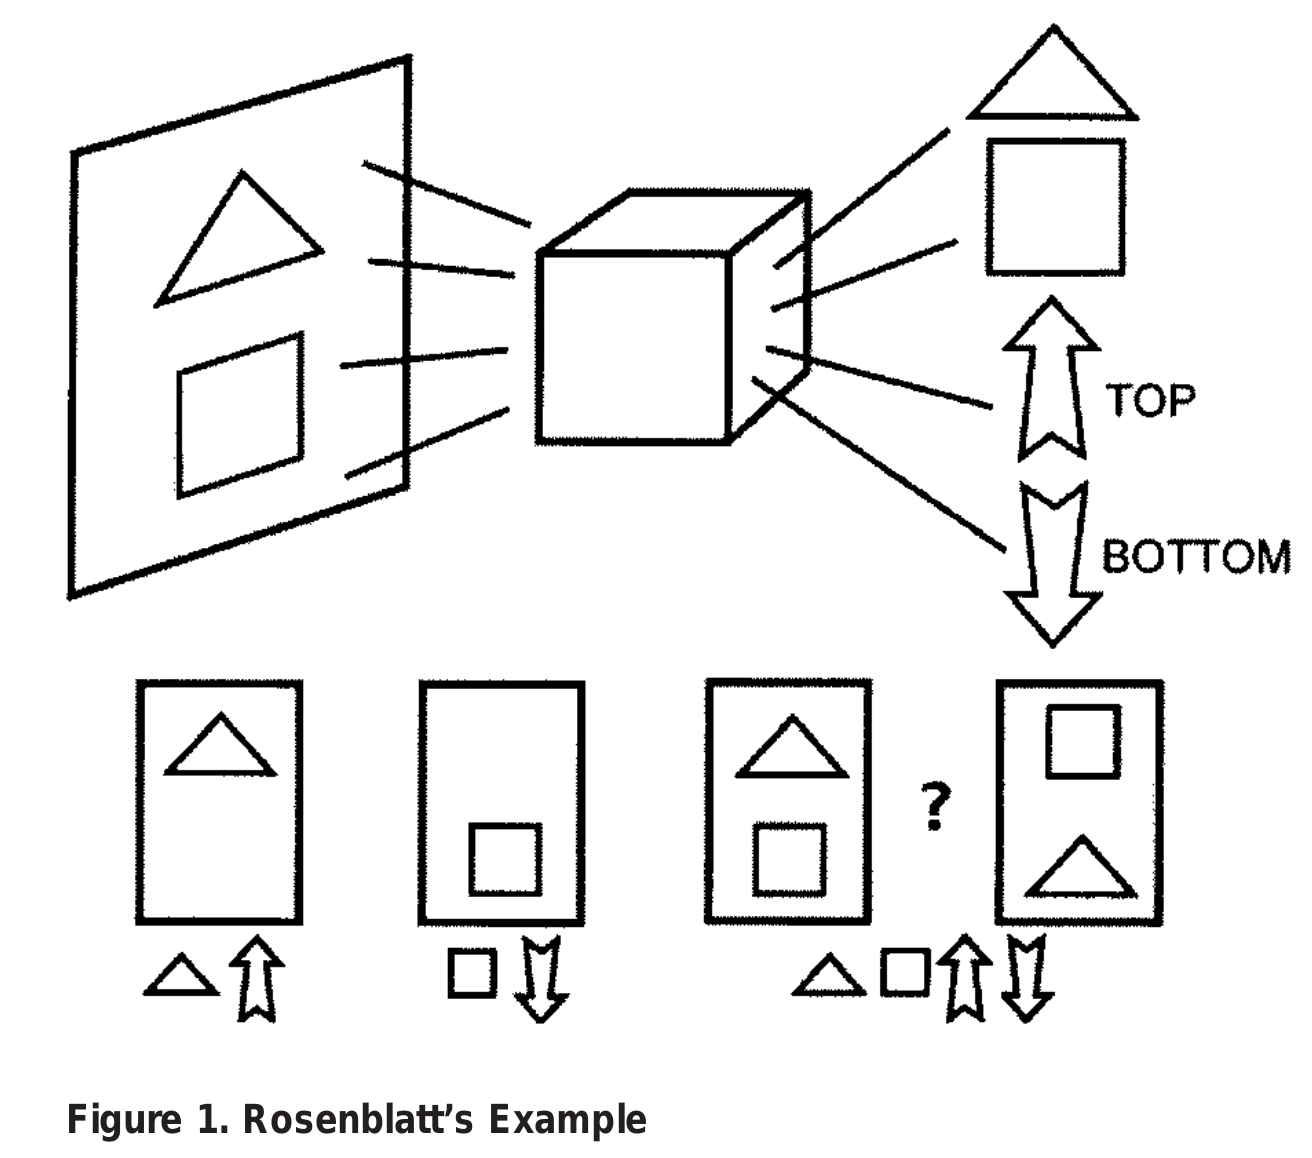
\includegraphics[width=1\textwidth]{the_binding_problem.png}
            {\tiny Необходимое количество узлов сети в такой схеме кодирования растет экспоненциально
            и требует значительно большего количества нейронов, чем наблюдается}
        \end{column}
        \begin{column}{0.6\textwidth}
            \emph{\footnotesize
                ``Although there is a widespread and more or less explicit
                conviction that classical neural networks are universal
                (in the sense, “give me a concrete problem and I will
                devise a network that solves it”), there is no basis for this
                claim whatsoever.

                ...Thus, the issue
                remains to identify in the brain a neural architecture that
                has the capacity for learning and self-organization and
                is a fertile basis for all the flexibility and creativity observed in humans and animals.''
            }

        {\tiny\cite{VonDerMalsburg1999}}
        \end{column}
    \end{columns}

\end{frame}

\begin{frame}[t]{\small Пресинаптический и постсинаптический потенциалы}{и их роль в передаче сигнала между нейронами. Осцилляции.}
\begin{columns}
    \begin{column}{0.5\textwidth}
        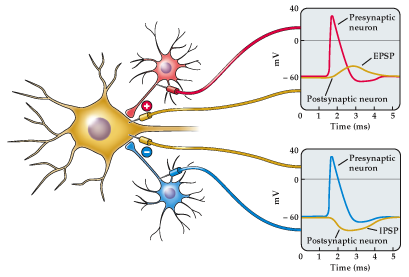
\includegraphics[scale=0.37]{neuronal_population.png}

        % \includegraphics[scale=0.3]{rythms.jpg}
    \end{column}

    \begin{column}{0.5\textwidth}
        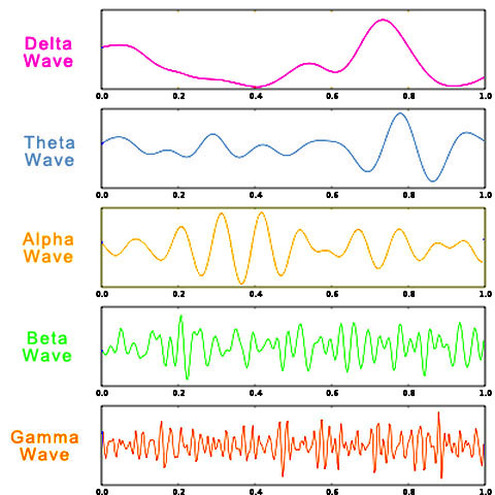
\includegraphics[width=5cm, height=7cm]{waves.jpg}
    \end{column}

    % \begin{column}{0.3\textwidth}
    % 	\includegraphics[scale=0.2]{pictures/rythms.jpg}
    % \end{column}

\end{columns}


\end{frame}

\begin{frame}[t]{\small Суммарный постсинаптический потенциал --- }{источник сигнала МЭГ/ЭЭГ}

    % Where does the signal come from?
    % Why we don't detect spikes.
    % Apical dendrites and neural activity summation.
    % Neocortex --- primary source of signal in MEG/EEG.
    % How many neurons produce detectable activation?

    % 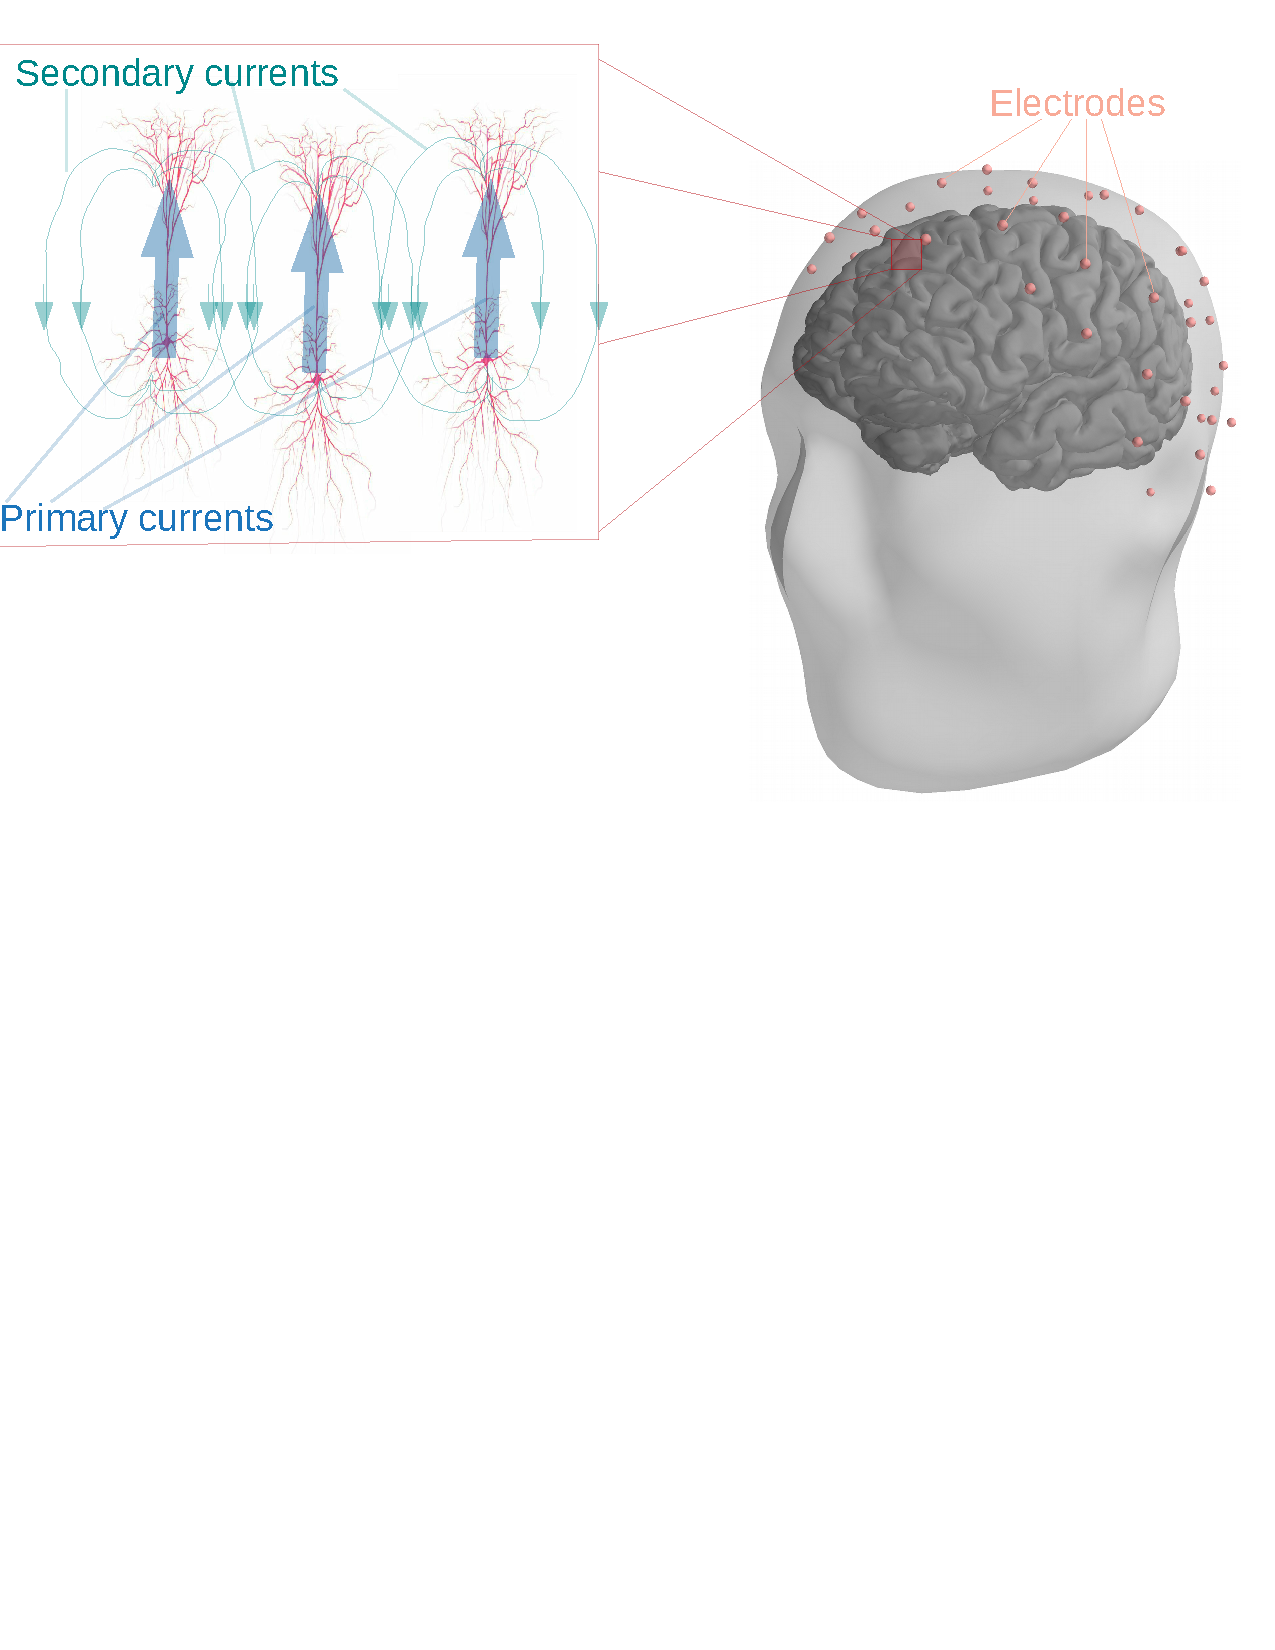
\includegraphics[width=1\textwidth]{../images/neuron.pdf}
    % \includegraphics[height=7cm, width=11.3cm]{../images/signal_src.pdf}
    \includegraphics[width=1\linewidth]{signal_src.pdf}
    {\tiny\cite{Baillet}}
    % 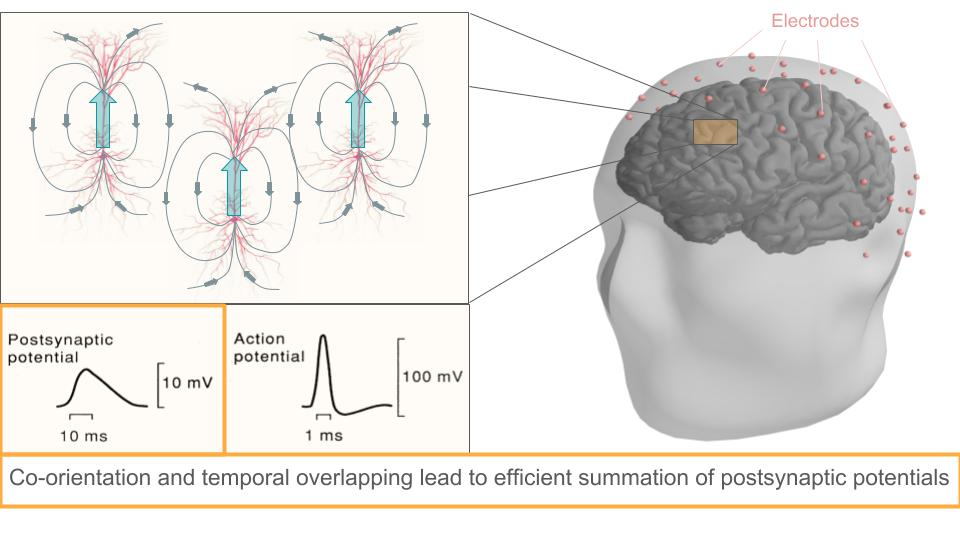
\includegraphics[width=1.05\textwidth]{../images/signal_src.jpg}
    % 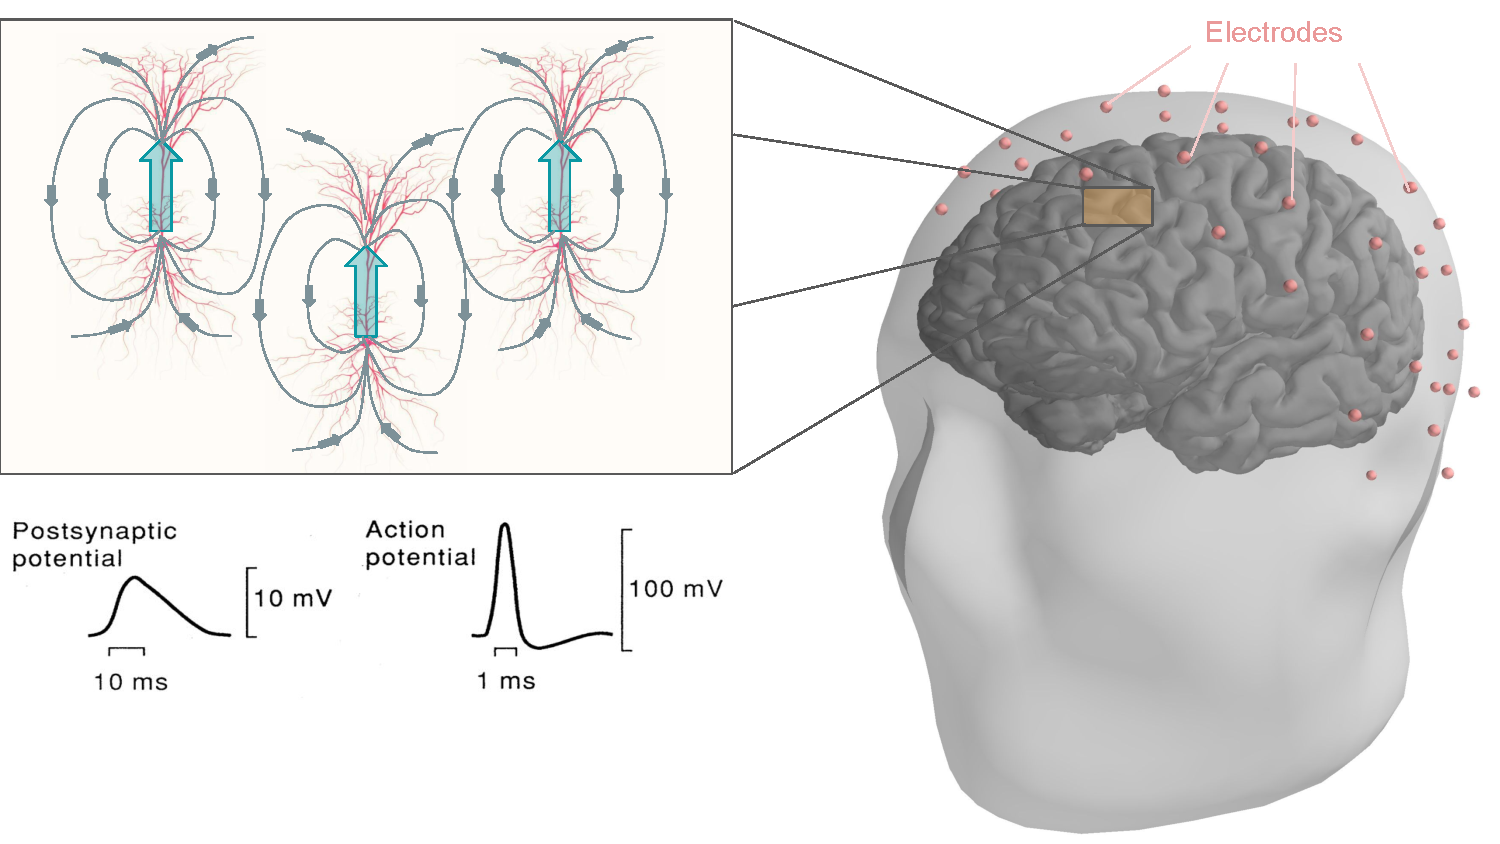
\includegraphics[width=1\textwidth]{../images/test.pdf}
    
    % 
\includegraphics[width=0.3cm]{battery_crp.jpg}
    % $\approx$ 1 million active synapses or $\approx$ 40 $mm^2$ of active cortex
    % needed to produce detectable activation in MEG {\tiny\cite{Hamalainen1993}}
\end{frame}

\begin{frame}{Гипотеза взаимодействия через когерентность}
    % Networks and CTC concepts
    % \begin{itemize}
    

    {\footnotesize``\ldots anatomical connections are dynamically rendered effective or ineffective through the presence or absence of rhythmic synchronization \ldots'' {\tiny\cite{Bastos2015}}}

    {\footnotesize ``In the absence of coherence, inputs arrive at random phases of the excitability cycle and will have a lower effective connectivity. A postsynaptic neuronal group receiving inputs from several different presynaptic groups responds primarily to the presynaptic group to which it is coherent.'' {\tiny\cite{Fries2015}}}
    
    \centering
    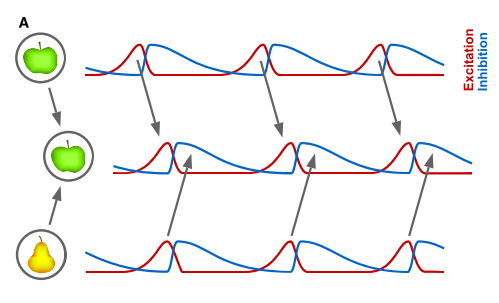
\includegraphics[scale=0.28]{CTC.png}
    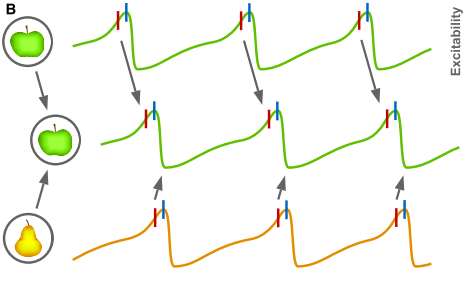
\includegraphics[scale=0.26]{CTC1.png}
    % {\tiny[Fries, 2015]}
\end{frame}

% Свидетельства наличия таких сетей
% Методы анализа синхронности
% Проблема объемной проводимости
% Imcoh
% Невозможность увидеть сети с нулевой фазой
% Проблема с восстановлением источников и измерением коннективности после
% Зачем нужен метод с прайорами
% Проблема протечки сигнала на уровне сетей

\begin{frame}[t]{Меры коннективности.}
    \centering
    \begin{columns}
        \begin{column}{0.5\textwidth}
            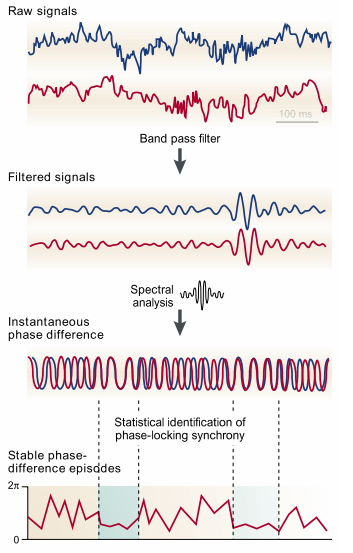
\includegraphics[scale=0.4]{phase_sunchrony.png}
        \end{column}
        \begin{column}{0.5\textwidth}
            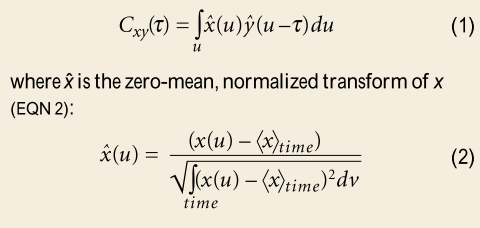
\includegraphics[scale=0.3]{correlation.png}

            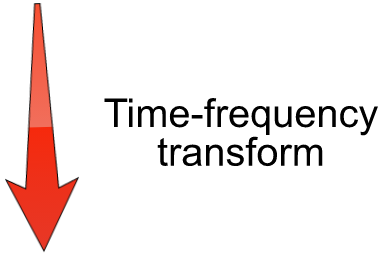
\includegraphics[scale=0.2]{tf_arrow.png}
            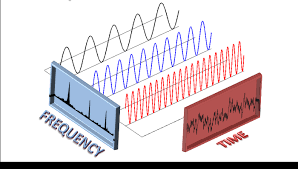
\includegraphics[scale=0.2]{time-frequency.png}

            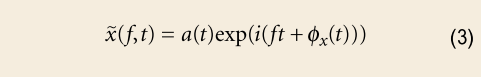
\includegraphics[scale=0.3]{eq3.png}

            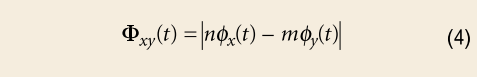
\includegraphics[scale=0.3]{eq4.png}
        \end{column}
        
    \end{columns}
    \vspace{-0.5cm}
    \hspace{5cm}{\cite{Varela2001}}
\end{frame}

\begin{frame}[t]
    \frametitle{Практическая значимость}
    \framesubtitle{мер коннективности}

    \vspace{2cm}
    \begin{columns}
        \begin{column}{0.5\textwidth}
            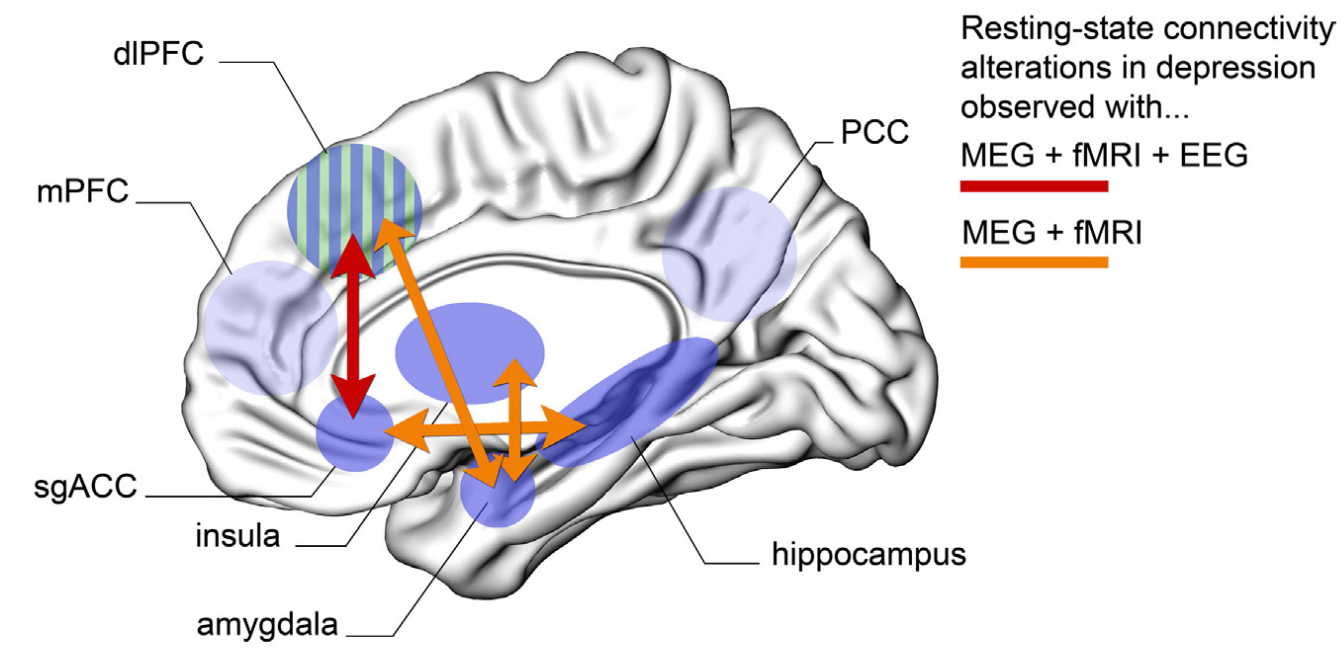
\includegraphics[width=1\textwidth]{alterations1.png}
            {\tiny Изменения коннективности при депрессии, \cite{Alamian_front2017}}
        \end{column}
        \begin{column}{0.5\textwidth}
            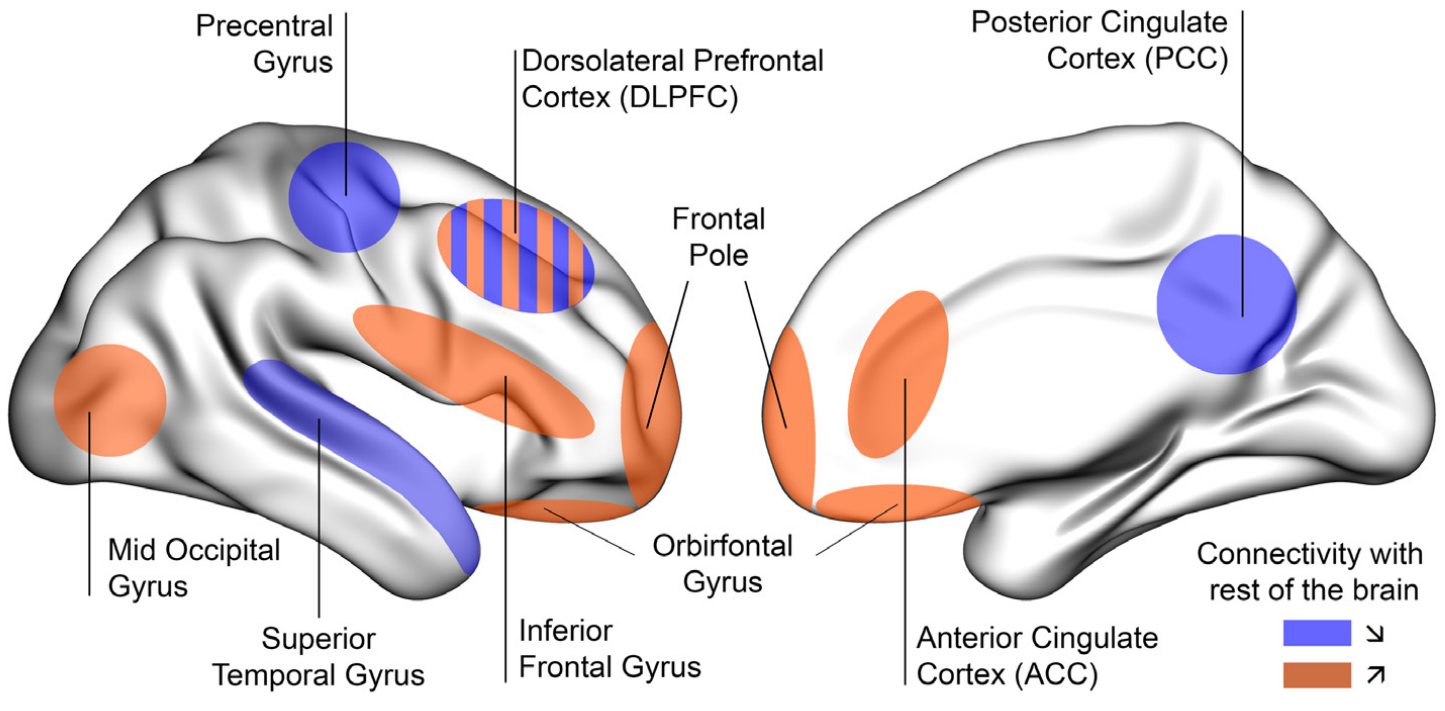
\includegraphics[width=\textwidth]{alterations2.png}
            {\tiny Изменения коннективности при шизофрении, \cite{Alamian_clin2017}}
        \end{column}
        
    \end{columns}
\end{frame}

\begin{frame}{Проблема протечки сигнала}

        {\smallСовместная регистрация мозговой активности от различных источников приводит
        к ложной детекции коннективности.}

        \centering  
        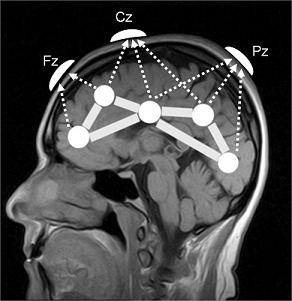
\includegraphics[scale=0.5]{head.png}
\end{frame}

\begin{frame}[t]
    \frametitle{Ложные (``призрачные'') взаимодействия}
    \vspace{1cm}
    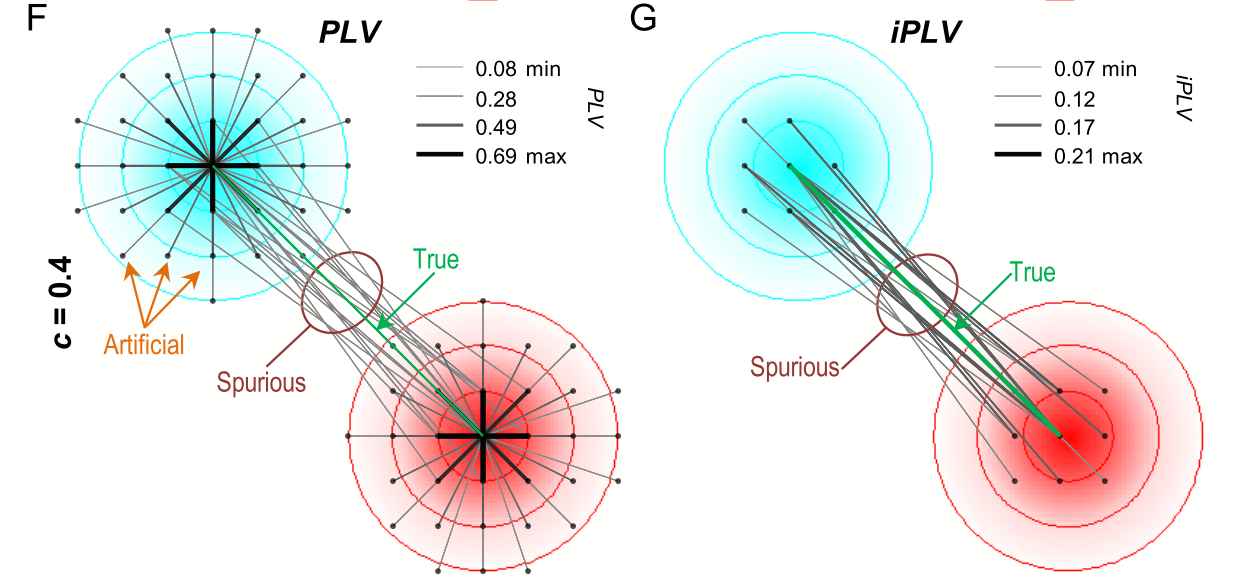
\includegraphics[scale=0.5]{karim_ghost_interactions.png}
    \cite{Palva2018}
\end{frame}

\begin{frame}[t]
    \frametitle{\small Подверженность ложным и артефактным взаимодействиям}
    \vspace{1cm}
    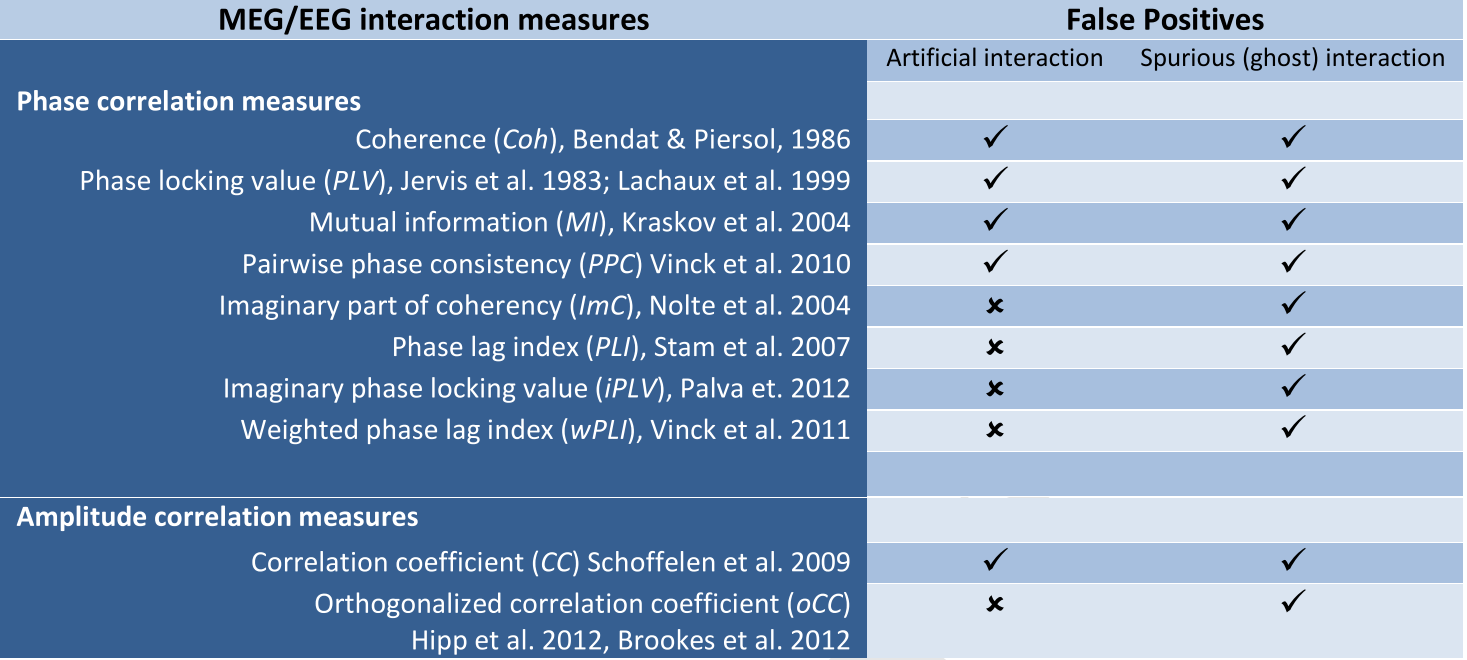
\includegraphics[width=\textwidth]{karim_table.png}
    \cite{Palva2018}
\end{frame}

\begin{frame}[t]{Недостатки существующих методов}{оценки коннективности}
    \begin{itemize}
        \footnotesize
        \item Часть методов игнорирует проблему протечки сигнала и потому подвержена
            артефактным детекциям сетей.
        \item Для методов, устойчивых к протечке сигнала, робастность достигается ортогонализацией временных рядов, что делает фазовую синхронизацию с малыми задержками невидимой и удаляет часть полезного сигнала.
            (Единственный метод, для которого это не так (GCS,~\cite{Wens2015}),
            никак не учитывает вклад третьих источников в протечку сигнала и потому на практике работает неудовлетворительно)
        \item Все имеющиеся методы неустойчивы к ``призрачным взаимодействиям''.
        \item При двухступенчатой оценке коннективности на уровне источников используются методы решения
            обратной задачи, функционал качества которых не предназначен для оценки коннективности.             Т.е. они в общем случае субоптимальны.
    \end{itemize}
\end{frame}

\begin{frame}[t]
    \frametitle{Цели исследования}
    
 Разработка метода оценки коннективностей, который:
\begin{itemize}
        \item позволяет оценить фазовую синхронность в условиях взаимной протечки сигналов
        \item чувствителен в том числе к сетям с малыми фазовыми задержками
        \item оптимален с точки зрения оценки достаточной статистики для коннективности
        \item способен учитывать априорную информацию об организации фазовых синхронностей
        \item не чувствителен к протечке сигнала на уровне сетей
\end{itemize}
а также его валидация в применении к симуляционным и реальным МЭГ-данным.
\end{frame}

% \begin{frame}{Эпохи}
%     \begin{columns}
%         \begin{column}{0.5\textwidth}
%             {\smallИспытуемому раз за разом предъявляют стимул, измеряя его мозговую активность.
%         Усреднение по таким повторениям позволяет сократить шум в данных}

%             \includegraphics[scale=0.25]{eeg_signal.png}
%         \end{column}
%         \begin{column}{0.5\textwidth}
%             \includegraphics[scale=0.25]{erp.jpg}

%             \includegraphics[scale=0.2]{evoked_topo.png}
%         \end{column}
%     \end{columns}
% \end{frame}

\begin{frame}[t]
    \frametitle{Проекция от протечки сигнала}
    
{\tiny Порождающая модель данных МЭГ/ЭЭГ для $k$-го предъявления стимула:}
\begin{equation}
    \scriptstyle
    \mathbf{x}_k(t) = \mathbf{G} \cdot \mathbf{s}_k(t) + \mathbf{\omega}_k(t),
    \label{gm_ts}
\end{equation}
{\tiny где $\mathbf{s}_k(t)$ ---  вектор активаций источников,
$\mathbf{x}_k(t)$ --- вектор сигналов на сенсорах,
$t$ --- время, а $\mathbf{G}$ --- матрица прямой модели.}

{\tiny Применим к данным частотно-временное преобразование (напр. преобр. Фурье с окном):}
\begin{equation}
    \scriptstyle
    \hat{\mathbf{x}}_k(f, t) = \mathbf{G} \cdot \hat{\mathbf{s}}_k(f, t) + \hat{\mathbf{\omega}}_k(f, t)
    \label{gm_timefreq_no_fi}
\end{equation}
{\tiny После частотно-временного преобразования порождающая модель кросс-спектра запишется как}
\begin{gather*}
    \scriptstyle
      \Cp{x}(f, t)  =  \langle{\hat{\mathbf{x}}_k(f, t) \hat{\mathbf{x}}_k(f, t)^{\dag}} \rangle_{k=1}^K =\\
    \scriptstyle
      = \langle{(\mathbf{G} \cdot\hat{\mathbf{s}}_k(f, t) + \hat{\mathbf{\omega}}_k(f, t))
                                       (\mathbf{G} \cdot\hat{\mathbf{s}}_k(f, t) + \hat{\mathbf{\omega}}_k(f, t))^{\dag}}\rangle_{k=1}^K=\nonumber\\
    \scriptstyle
     = \sum\limits_{p=1}^n\sum\limits_{q=1}^n\mathbf{g}_p\mathbf{g}_q^T c_{pq}^{\mathbf{ss}}(f, t) + \Cp{\omega}(f, t)
% =
% \mathbf{G}  \cdot \langle{\hat{\mathbf{s     }}_k(t) \hat{\mathbf{s     }}_k(t)^{\dag}} \rangle_{k=1}^K \cdot \mathbf{G}^T +
%    \mathbf{G} \cdot \langle{\hat{\mathbf{s     }}_k(t) \hat{\mathbf{\omega}}_k(t)^{\dag}} \rangle_{k=1}^K + \nonumber\\
%         +  \langle{\hat{\mathbf{\omega}}_k(t) \hat{\mathbf{s     }}_k(t)^{\dag}} \rangle_{k=1}^K \cdot \mathbf{G}^T +
%            \langle{\hat{\mathbf{\omega}}_k(t) \hat{\mathbf{\omega}}_k(t)^{\dag}} \rangle_{k=1}^K,
    \label{gm_cp_ini}
\end{gather*}
     {\tiny Векторы вида $\mathbf{g}_p$ --- это столбцы матрицы $\mathbf{G}$. Их принятно называть топографиями источников.}
\end{frame}

\begin{frame}[t]
    \frametitle{Проекция от протечки сигнала}
    
\begin{gather}
    \scriptstyle
    \Cp{x}(t) = \sum\limits_{p=1}^n\sum\limits_{q=1}^n\mathbf{g}_p\mathbf{g}_q^T c_{pq}^{\mathbf{ss}}(t) + \Cp{\omega}(t)
    \label{cp_rhs_expanded}
\end{gather}

{\tiny Векторизуем уравнение \ref{cp_rhs_expanded}:}
\begin{equation}
    \scriptstyle
    vec(\Cp{x}(t)) = \sum\limits_{p=1}^n\sum\limits_{q=1}^n
    \mathbf{g}_q\otimes \mathbf{g}_p \cdot c_{pq}^{\mathbf{ss}}(t) + vec(\Cp{\omega}(t))
    \label{cp_rhs_kron}
\end{equation}
{\tiny Распишем мнимую и действительную часть нешумовой компоненты ур. \ref{cp_rhs_kron}:}

\begin{gather*}
    \scriptstyle
    vec(\Cp{x}(t)) = \\
    % Re\left(\sum\limits_{p,q=1}^{n,n} \mathbf{g}_q\otimes \mathbf{g}_p \cdot c_{pq}^{\mathbf{ss}}(t)\right) +
    %  i \cdot Im\left(\sum\limits_{p,q=1}^{n,n}
    %  \mathbf{g}_q\otimes \mathbf{g}_p \cdot c_{pq}^{\mathbf{ss}}(t)\right) = \nonumber \\
    \scriptstyle
           =2\sum\limits_{p}^{n} \mathbf{g}_p\otimes \mathbf{g}_p c_{pp}^{\mathbf{ss}}(t) +
           \sum\limits_{p< q}^{n,n} (\mathbf{g}_q\otimes \mathbf{g}_p + \mathbf{g}_p\otimes \mathbf{g}_q)
           Re\left(c_{pq}^{\mathbf{ss}}(t)\right) + \\
    \scriptstyle
     + i \cdot \sum\limits_{p<q}^{n,n} (\mathbf{g}_q\otimes \mathbf{g}_p - \mathbf{g}_p\otimes \mathbf{g}_q)
           Im\left(c_{pq}^{\mathbf{ss}}(t)\right) + vec(\Cp{\omega}(t))
    \label{eq:cp_re_im}
\end{gather*}
{\tiny Ветора вида $\mathbf{g}_q\otimes \mathbf{g}_p + \mathbf{g}_p\otimes \mathbf{g}_q$ будем называть \emph{2-топографиями.} Наша цель --- оценить $c_{pq}^{ss}$ по этому уравнению}

\end{frame}

\begin{frame}[t]
    \frametitle{Взаимосвязь подпространств}
    \framesubtitle{2-топографий мнимой части, действительной части и объемной проводимости}
    
    \begin{figure}[htbp]
    \centering
    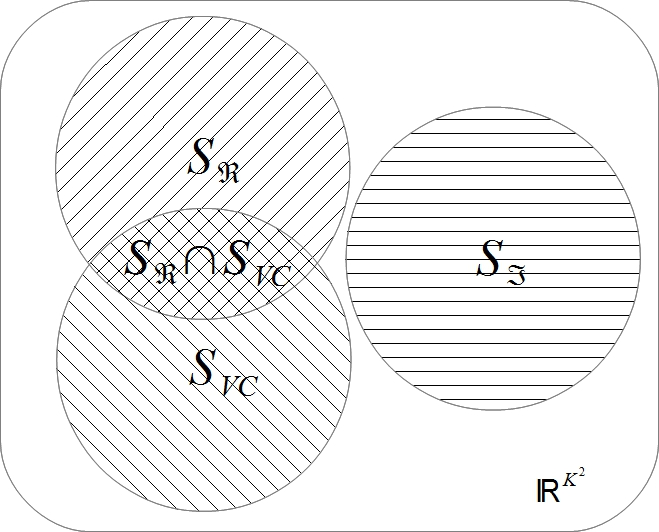
\includegraphics[width=0.5\textwidth]{SetsReImVC.jpg}

{\tiny Подпространство протечки сигнала $S_{SL}$ и подпространство действительной части кросс-спектра $S_{\Re}$
имеют непустое пересечение. Оба этих подпространства ортогональны подпространству мнимой
части кросс-спектра $S_{\Im}$.
Пересечение $S_{SL}$ с $S_{\Re}$ содержит вклад как от протечки сигнала,
так и от истинно взаимодействующих источников,
расположенных близко друг к другу и характеризующихся малой разностью фаз.}
\end{figure}%
\end{frame}

\begin{frame}[t]
    \frametitle{Проекция от протечки сигнала}
    
{\tiny 2-топографии $\mathbf{g}_q\otimes \mathbf{g}_q$ задают пространственную структуру протечки сигнала,
т.к. они отображают на сенсоры диагональные (мощностные) элементы кросс-спектра источников}

    {\tiny Рассмотрим матрицу, составленную из 2-топографий протечки сигнала:}

    \begin{equation}
        \scriptstyle
        \mathbf{F} =
        \begin{bmatrix}
            |                                 & |                                 &       & |                                 \\
            \mathbf{g}_1 \otimes \mathbf{g}_1 & \mathbf{g}_2 \otimes \mathbf{g}_2 & \dots & \mathbf{g}_n \otimes \mathbf{g}_n \\
            |                                 & |                                 &       & |
        \end{bmatrix}
    \end{equation}

    {\tiny Произведем сингулярное разложение матрицы $\mathbf{F}$}:
\begin{equation}
    \scriptstyle
    \mathbf{F} = \mathbf{USV}^T
\end{equation}
    {\tiny Для построения проектора используем $r$ левых собственных векторов:}

\begin{equation}
    \scriptstyle
    \mathbf{P}_r = \mathbf{I} - \mathbf{U}_r \mathbf{U}_r^T\label{eq:P_fixed_or};\quad
    \mathbf{U}_r =
    \begin{bmatrix}
        |            & |            &        & |       \\
        \mathbf{u}_1 & \mathbf{u}_2 & \dots  & \mathbf{u}_r \\
        |            & |            &        & |
    \end{bmatrix}\label{eq:U_fixed_or};
 \end{equation}
\end{frame}


\begin{frame}[t]
    \frametitle{Взаимная протечка сигнала}
{\tiny Определим ядро разрешения метода решения обратной задачи (\cite{Sekihara2007}):}
    
\begin{equation}
    \scriptstyle
    R(i, k) = \vec{l}_i^T \vec{g}_k
    \label{eq:resolution_kernel}
\end{equation}
{\tiny $\vec{l}_i$~--- фильтр в направлении $i$-ой точки коры, а
$\vec{g}_j$~--- топография точки коры с индексом $k$}

{\tinyДля совокупности $N$ точек коры можно определить функцию
$\vec{B}(i)$. Она имеет смысл протечки сигнала от каждой точки коры в
фиксированную точку $i$ (~\cite{Sekihara2007}).}
\begin{equation}
    \scriptstyle
    \vec{B}{(i)}^T = \left[R{(i, 1)}, R(i, 2), \ldots, R(i, N)\right]
\end{equation}

{\tiny Назовём \emph{взаимной протечкой сигнала} для точек $i$, $j$ скалярное произведение вида:}
\begin{equation}
    \scriptstyle
    \mu(i, j) \defeq {(\vec{B}{(i)}^{\odot 2})}^T \vec{B}{(j)}^{\odot 2}
    \label{eq:def_mutual_leakage}
\end{equation}
{\tiny Здесь операция ${(\cdot)}^{\odot 2}$ означает поэлементное возведение в квадрат.}
\end{frame}


\begin{frame}[t]
    \frametitle{Метод PSIICOS}

    \vspace{1cm}

    \underline{Утверждение.}
    \vspace{3mm}

    {\footnotesize Фильтры вида}
    \begin{equation}
        \vec{v}_{ij} = \frac{\matr{P} ( \mathbf{g}_i\otimes \mathbf{g}_j) } { \norm{\matr{P}( \mathbf{g}_i\otimes \mathbf{g}_j)}^2 },
        \label{eq:min_leakage_solution}
    \end{equation}
    {\footnotesize действующие на векторизованный кросс-спектр на уровне сенсоров, дают оценку
        элемента $c_{ij}^{\mathbf{ss}}$ кросс-спектра на уровне источников, с минимальной взаимной протечкой сигналов
    $\mu(i, j)$ среди всех фильтров с единичным усилением для сети $i, j$.

    \vspace{3mm}
    Методом PSIICOS мы назваем метод оценки элементов кросс-спектра на источниках
при помощи пространственных фильтров вида (\ref{eq:min_leakage_solution}), (Ossadtchii, Altukhov, Jerbi [2018])}
    
\end{frame}

\begin{frame}[t]
    \frametitle{Метод PSIICOS Unbiased}
    Полученные фильтры приводят к пространственно смещенным оценкам.
    Чтобы исправить эту проблему, мы модифицируем метод PSIICOS, вводя иную
    нормировку фильтров:
    
\begin{gather*}
    \vec{v}_{ij}^{Re} = \frac{2\matr{P}\vec{q}_{ij}}{\norm{\matr{P}(\vec{q}_{ij} + \vec{q}_{ji})}}\\
    \vec{v}_{ij}^{Im} = \frac{2\vec{q}_{ij}}{\norm{\vec{q}_{ij} - \vec{q}_{ji}}}
\end{gather*}
    где $\vec{q}_{ij} = \mathbf{g}_j\otimes \mathbf{g}_i$.

    Мы показываем, что такая нормировка дает пространственно несмещенные оценки.
    Эту модификацию метода мы называем PSIICOS Unbiased.
\end{frame}

\begin{frame}{GO-PSIICOS}
    \begin{block}{\tiny Уравнения на коэффициенты $c_{ij}^{SS}$ выглядят как:}
  \begin{equation}
      \scriptstyle
      \mathbf{P}vec(\mathbf{C}(t)) = {\sum\limits_{i=1}^{L}\sum\limits_{j=1}^{L}}\mathbf{P}vec(\mathbf{g_{i}g_{j}^T}){c_{ij}^{ss}(t)} + vec(\mathbf{C^{NN}}(t))
      \label{eq9}
  \end{equation}
 \end{block}
 \begin{block}{\tinyОпределим новые переменные:}
     \tiny
     $\mathbf{\Omega}(t) \defeq \mathbf{P}vec(\mathbf{C}(t))$,
     $\mathbf{\Gamma_{k}} \defeq \mathbf{P}vec(\mathbf{g_{i}g_{j}^T}),\, \mathbf{\sigma_{k}}(t) = c_{ij}^{ss}(t), \mathbf{N}(t) = \mathbf{C^{NN}}(t)$; тогда (\ref{eq9}) перепишется
  \begin{equation}
   \label{eq10}
   \mathbf{\Omega}(t) = {\sum\limits_{k=1}^{L^{2}}}\mathbf{\Gamma_{k}\sigma_{k}}(t) + \mathbf{N}(t)
  \end{equation}
 \end{block}

 \begin{block}{\tiny Оптимизационный критерий метода GO-PSIICOS:}
     \tiny
  % \begin{equation}
  %     \scriptstyle
  %  \frac{1}{2}\norm{\mathbf{\Omega}(t) - {\sum\limits_{k=1}^{{L^{2}}}}\mathbf{\Gamma_{k}\sigma_{k}}(t) }_{Fro}^{2} +\lambda{\sum\limits_{k=1}^{L^2}}\sqrt{\norm{\mathbf{\sigma_{k}}(t)}}_{Fro} \longrightarrow min
  %  \end{equation}
   \begin{equation}
    \frac{1}{2}\norm{\mathbf{\Omega} - \mathbf{\Gamma \Sigma}}_{Fro}^{2} +\lambda{\sum\limits_{k=1}^{L^2}}\sqrt{\norm{\mathbf{\Sigma}_{k}}}_{Fro} \longrightarrow min
   \end{equation}
 \end{block}
\end{frame}

\begin{frame}{Выбор регуляризации со смешанной нормой}
 Регуляризационное слагаемое
 {${\sum\limits_{k=1}^{L^2}}\sqrt{\norm{\mathbf{\Sigma}_{k}}}_{Fro}$}
 задает штраф с псевдонормой $l_{2,0.5}$.
 \begin{figure}
 \centering
 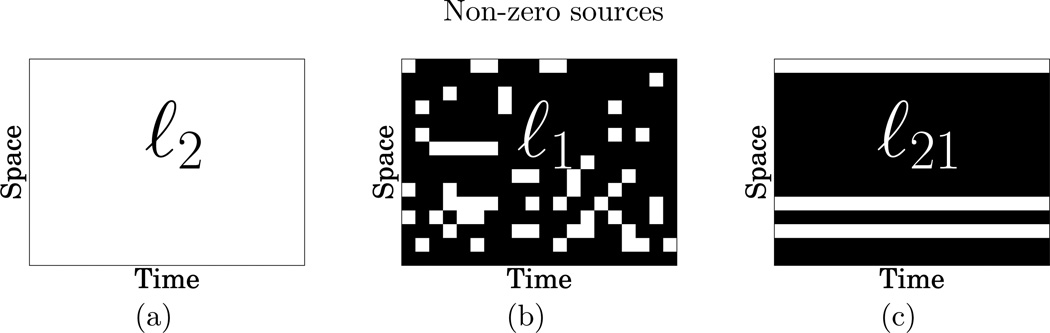
\includegraphics[scale = 0.5]{Mixed-norm.jpg}

 {\footnotesize Структура решений для различных видов штрафующей нормы (\cite{Gramfort2012})}
 \label{fig:mix_n}
 \end{figure}
\end{frame}

\begin{frame}[t]{Влияние проекции на нормы 2-топографий}
    % \frametitle{title}
    \begin{figure}[!ht]
     \centering
     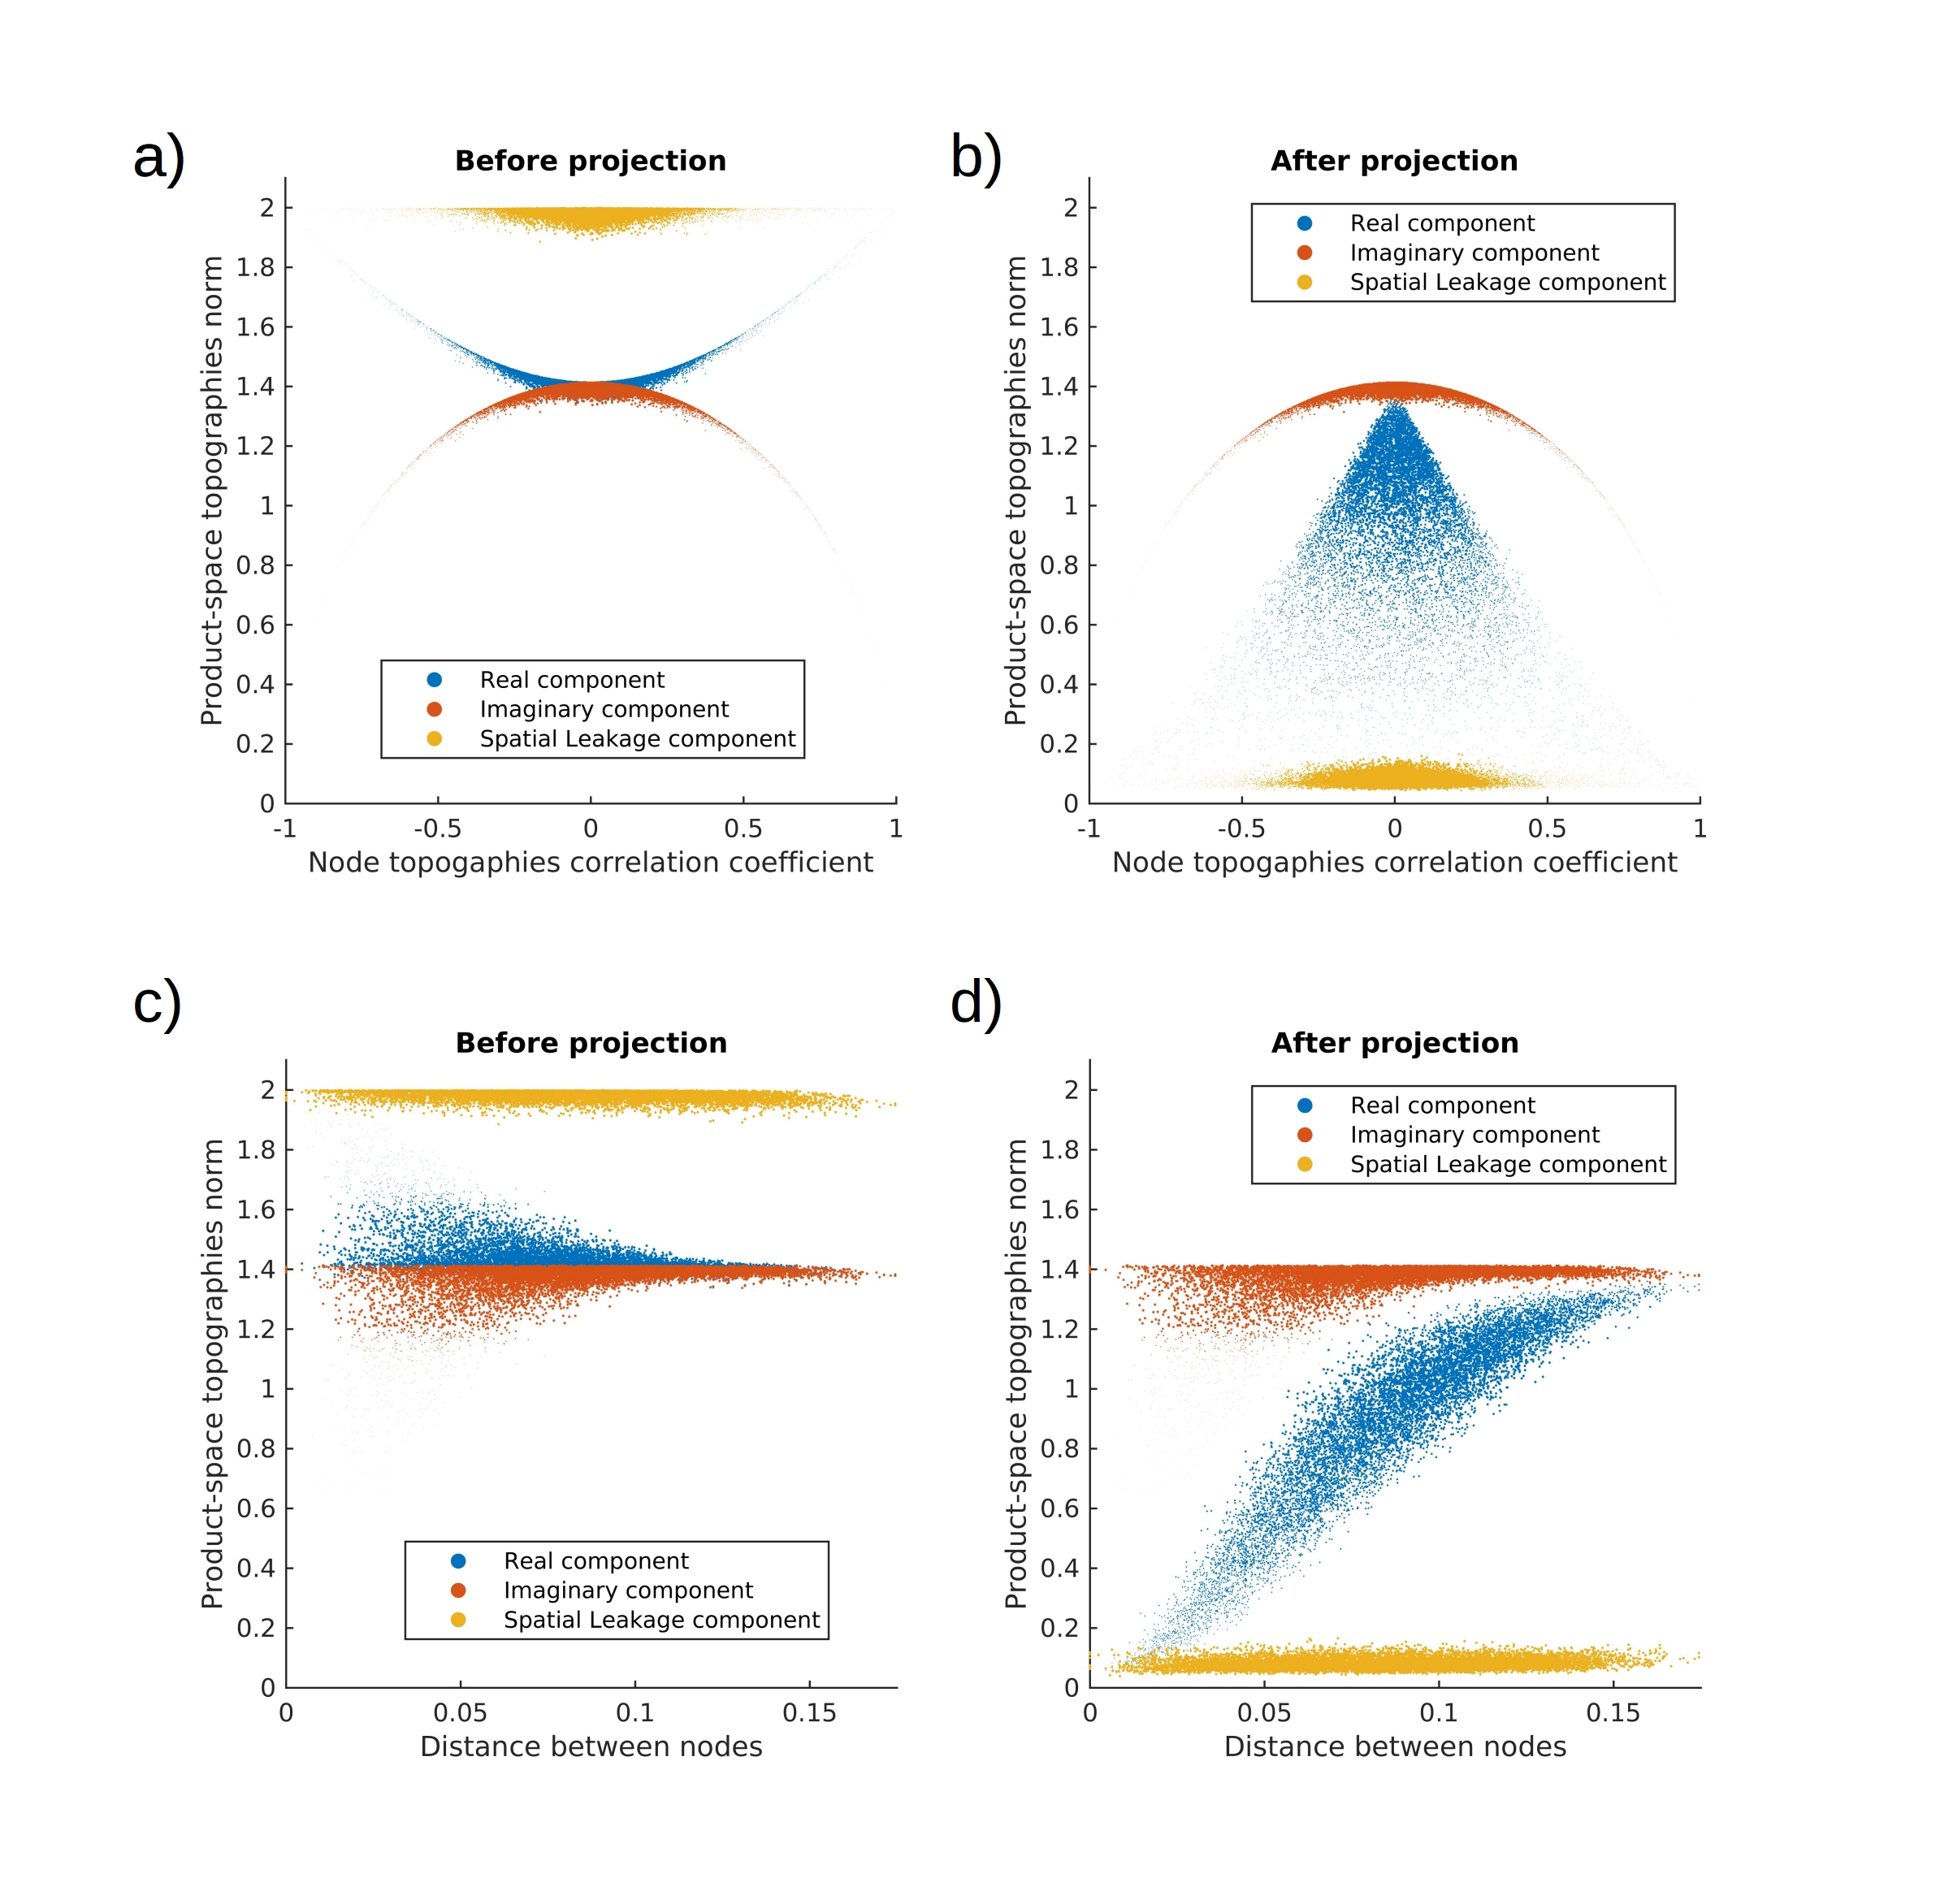
\includegraphics[width=0.7\textwidth, height=6cm]{../images/psiicos_paper/Figure3abcd_hr}

     {\tiny Нормы 2-топографий для трех подпространств кросс-спектра до и после проекци
         в зависимости от коэффициента корреляции топографий (графики (a) и (b)), и от расстояния между узлами (графики (c) и (d)).}
         % До проекции (графики (a), (c)) в кросс-спектр на уровне сенсоров наибольший вклад дает мощностная
         % компонента (обозначена желтым цветом). После проекции (графики (b), (d))
         % вклад мощностной компоненты уменьшается в среднем в 25 раз. Вместе с
         % тем наблюдается неизбежное, но значительно меньшее ослабление
         % 2-топографий действительной части, соответствующих истинной коннективности.
         % В среднем они ослабляются в 1.6 раз.
    \end{figure}
\end{frame}

\begin{frame}[t]
    \frametitle{Симуляцонные данные}
    \begin{columns}
        \begin{column}{0.6\textwidth}
            \begin{block}{\tinyОбщие параметры симуляций}
                \begin{itemize}
                    \tiny
                    \item Индуцированная активность на частоте 10 Гц
                    \item 1000 источников мозгового шума со случайными и разными
                        для каждой эпохи положениями на коре
                    \item Спектр мозгового шума моделировался в соответствии с профилем 1/f
                    \item Истинные источники задавались на сетке 15000 узлов,
                        а восстанавливались на сетке 1500 узлов
                    \item Для целевых сетей задавалась фазовая связность с варьируемым
                        средним фазовым сдвигом $\phi$ и постоянным разбросом фазового сдвига $\alpha$
                    \item Отношение сигнал-шум для целевых сетей варьировалось
                    \item Детекция сети считалась корректной при попадании обоих узлов
                        в шар радиусом 1.5 см с центром в истинном положении
                \end{itemize}
            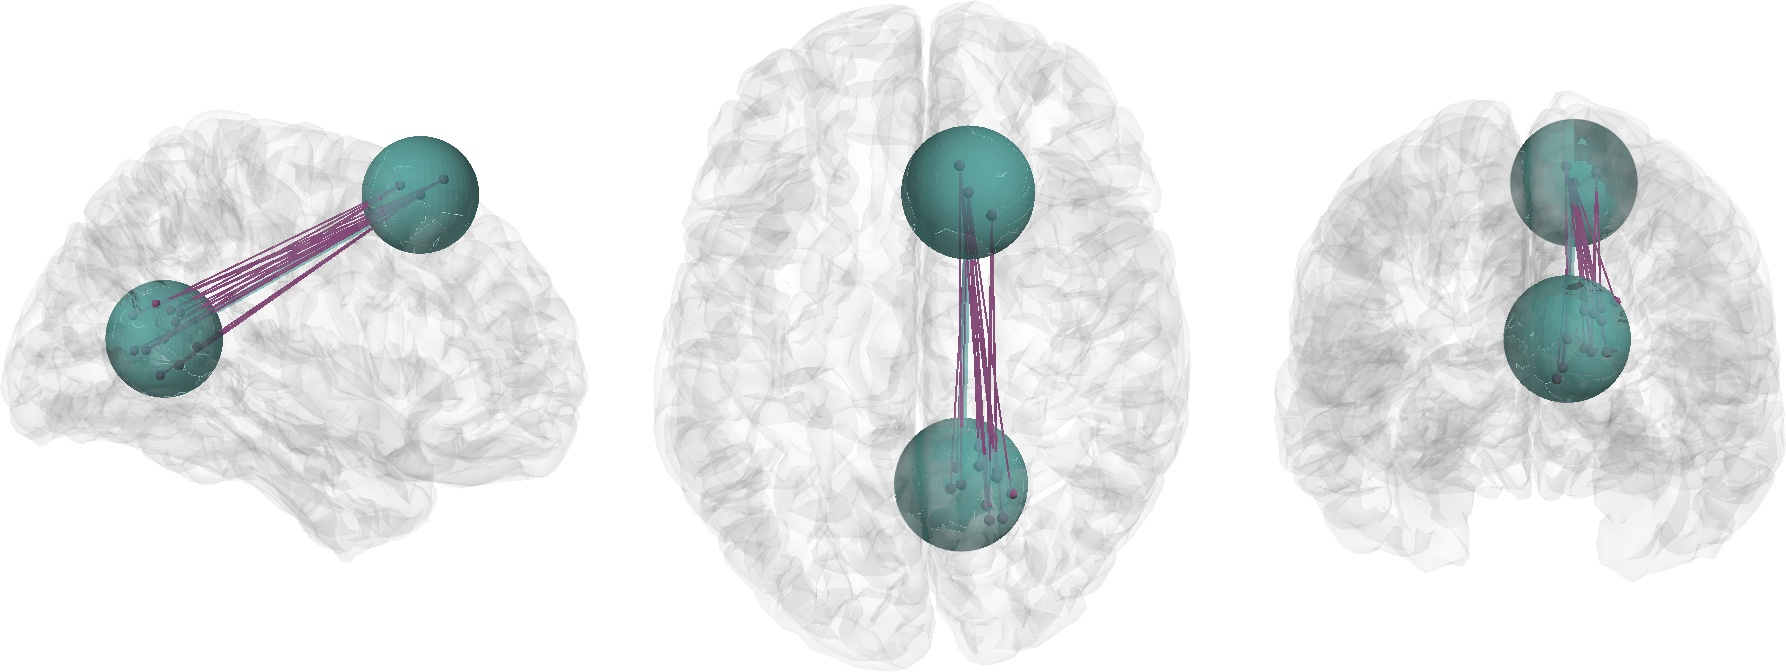
\includegraphics[width=0.99\textwidth]{../images/bias_brain_PSIICOS_Unbiased.jpg}
            \end{block}
            
        \end{column}
        \begin{column}{0.4\textwidth}
            \begin{block}{\tinyСимуляции с тремя перекрывающимися во времени сетями}
                \begin{itemize}
                    \tiny
                    \item Положения узлов фиксированные
                \end{itemize}
            \centering
            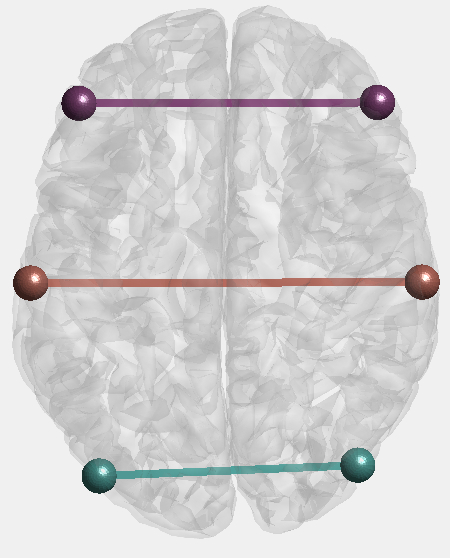
\includegraphics[angle=90, width=0.5\textwidth]{../images/psiicos_paper/Figure2a_hr.jpg}
            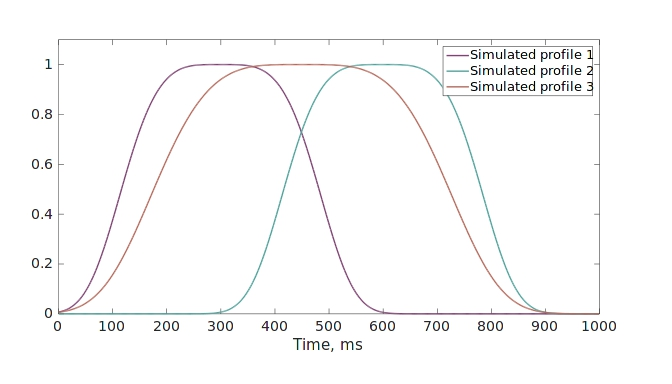
\includegraphics[width=0.6\textwidth]{../images/psiicos_paper/Figure2b_hr.jpg}
            \end{block}
            \begin{block}{\tinyСимуляции со случайными положениями узлов}
                \begin{itemize}
                    \tiny
                    \item Положения узлов выбирались случайно N раз (симуляции Монте-Карло)
                    \item Для каждого из N повторений вычислялась метрика качества, результат усреднялся.
                \end{itemize}
            \end{block}
        \end{column}
    \end{columns}
\end{frame}

\begin{frame}[t]{Влияние фазового сдвига}{на качество решений для алгоритма PSIICOS}
    % \framesubtitle{subtitle}
    
    \begin{figure}[!ht]
     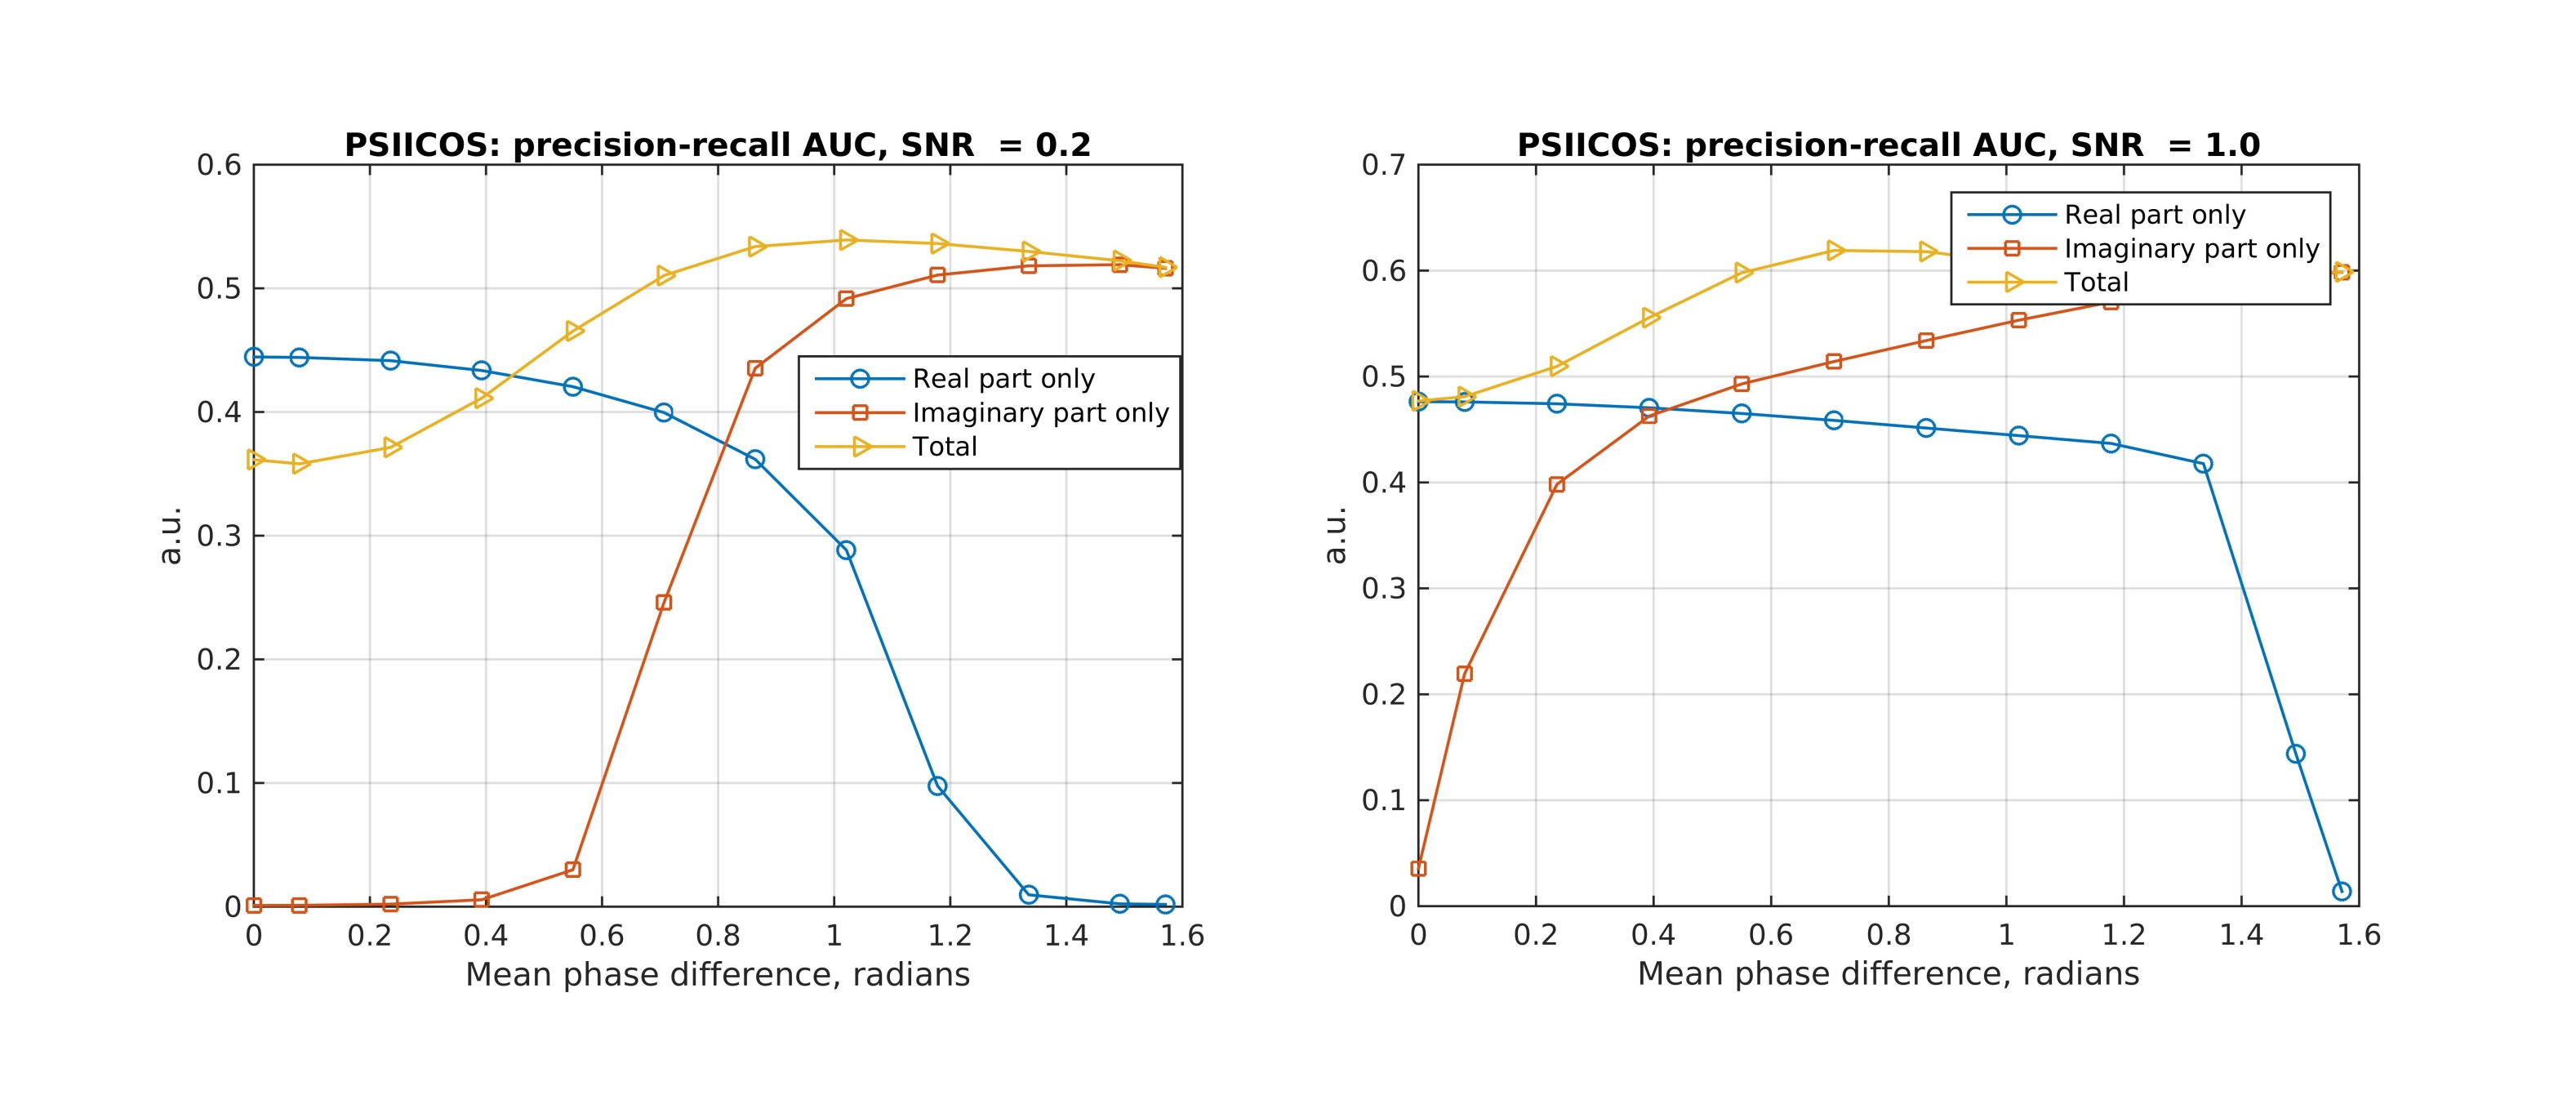
\includegraphics[width=1\textwidth]{../images/psiicos_paper/Figure9_hr.jpg}
     {\tiny Метрики качества решения алгоритма PSIICOS в зависимости от средней фазовой задержки в задаче
     с тремя сетями}
         % (a)~--- для низкого значения ОСШ и (b)~--- для высокого.
         % Для близких к $\pi/2$ средних значений фазового сдвига информация
         % о взаимодействии источников содержится в основном во мнимой части кросс-спектра.
         % Поэтому использование только мнимой части (что эквивалентно iDICS) позволяет
         % достигать высокого качества решения; качество решения при этом затухает
         % с уменьшением фазового сдвига. С другой стороны, для близких к нулю
         % значений фазовой задержки информация о взаимодействии содержится в основном
         % в действительной части кросс-спектра. Действительная часть загрязнена
         % протечкой сигнала, которая может быть удалена при помощи PSIICOS-проекции.
         % После этого очищенная действительная часть используется для обнаружения
         % сетей с близкими к нулю фазовыми задержками (синие кривые). Одновременное
         % использование действительной и мнимой компоненты позволяет добиться равномерного
         % качества решений по всему диапазону средних фазовых сдвигов (оранжевая кривая).
    \end{figure}% Figure 9
\end{frame}

\begin{frame}{Сравнение PSIICOS c GCS, DICS и iDICS}{для трех сетей со случайными положениями узлов}
 \begin{figure}[!ht]
 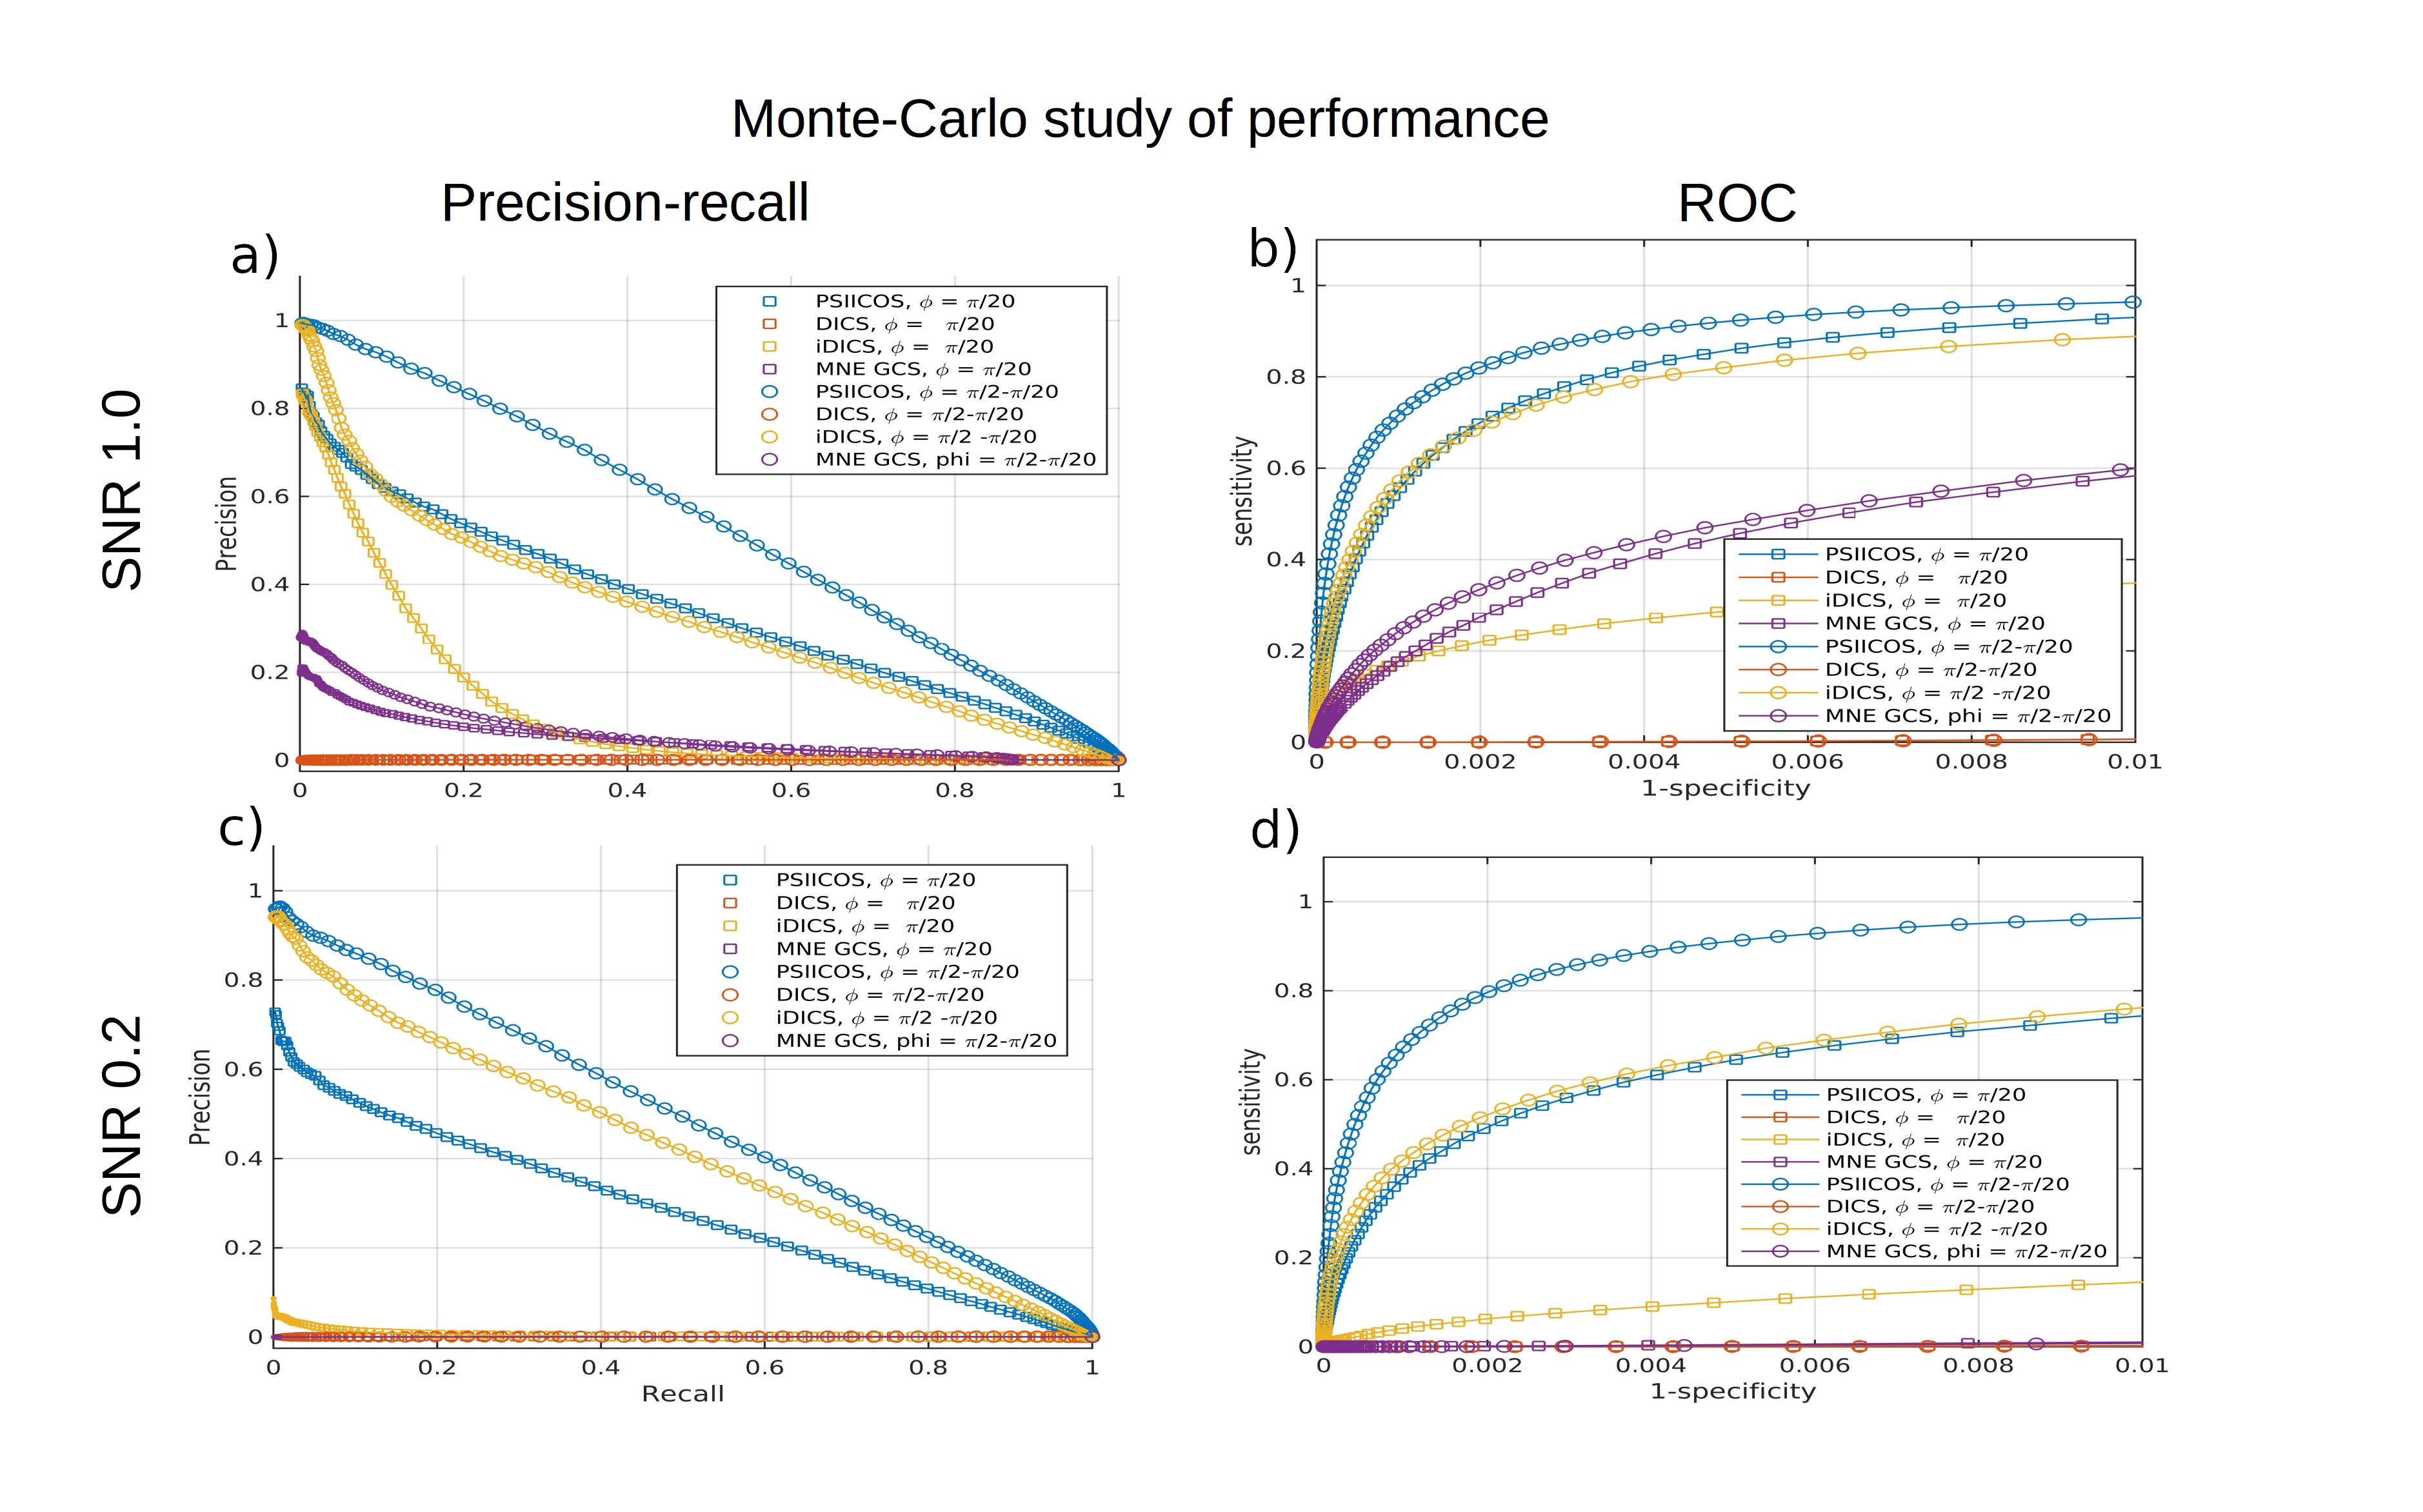
\includegraphics[width=1\textwidth]{../images/psiicos_paper/Figure4_hr_labelled_pans.jpg}
 % \caption{Сравнение Precision-Recall (панели (a), (c))  и ROC- (панели (b), (d)) кривых
 %     в задаче локализации сетей для методов PSIICOS, DICS, iDICS и GCS MNE для
 %     двух значений ОСШ на основе 1000 Монте-Карло итераций.}\label{fig:04} %Figure 4
\end{figure}%
\end{frame}


% \begin{frame}
% \frametitle{Симуляции сетей с перекрывающимися временными профилями}
% \begin{figure}[htbp]
%     \begin{columns}
%         \begin{column}{0.4\textwidth}
%             \centering
%         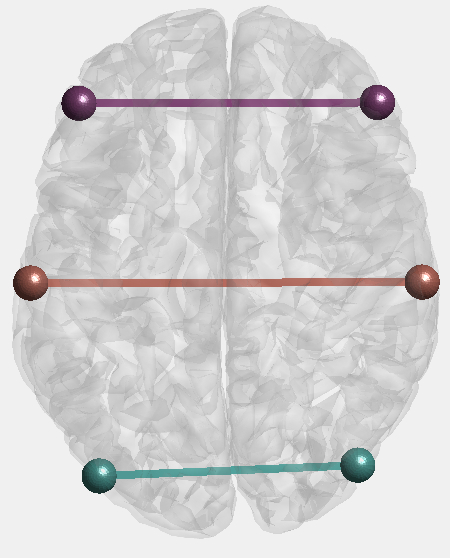
\includegraphics[angle=90, width=1\textwidth]{../images/psiicos_paper/Figure2a_hr.jpg}
%         {\small Пространственная конфигурация сетей}
%         \end{column}
%         \begin{column}{0.6\textwidth}
%             \centering
%             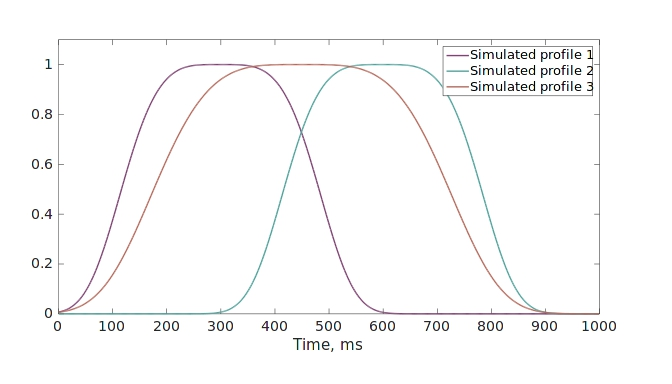
\includegraphics[width=1\textwidth]{../images/psiicos_paper/Figure2b_hr.jpg}
%         {\small Временные профили активации}
%         \end{column}
%     \end{columns}
%     % \caption{Три симулированные пары взаимодействующих источников.}\label{02}
%     %     (а)~--- пространственное распределение симулированных источников,
%     %     (б)~--- временные профили активации для каждой из трех сетей.
% \end{figure}
% \end{frame}

\begin{frame}
{Сравнение PSIICOS c GCS, DICS и iDICS}{для трех сетей с перекрывающимися профилями активации}
\begin{figure}[!ht]
 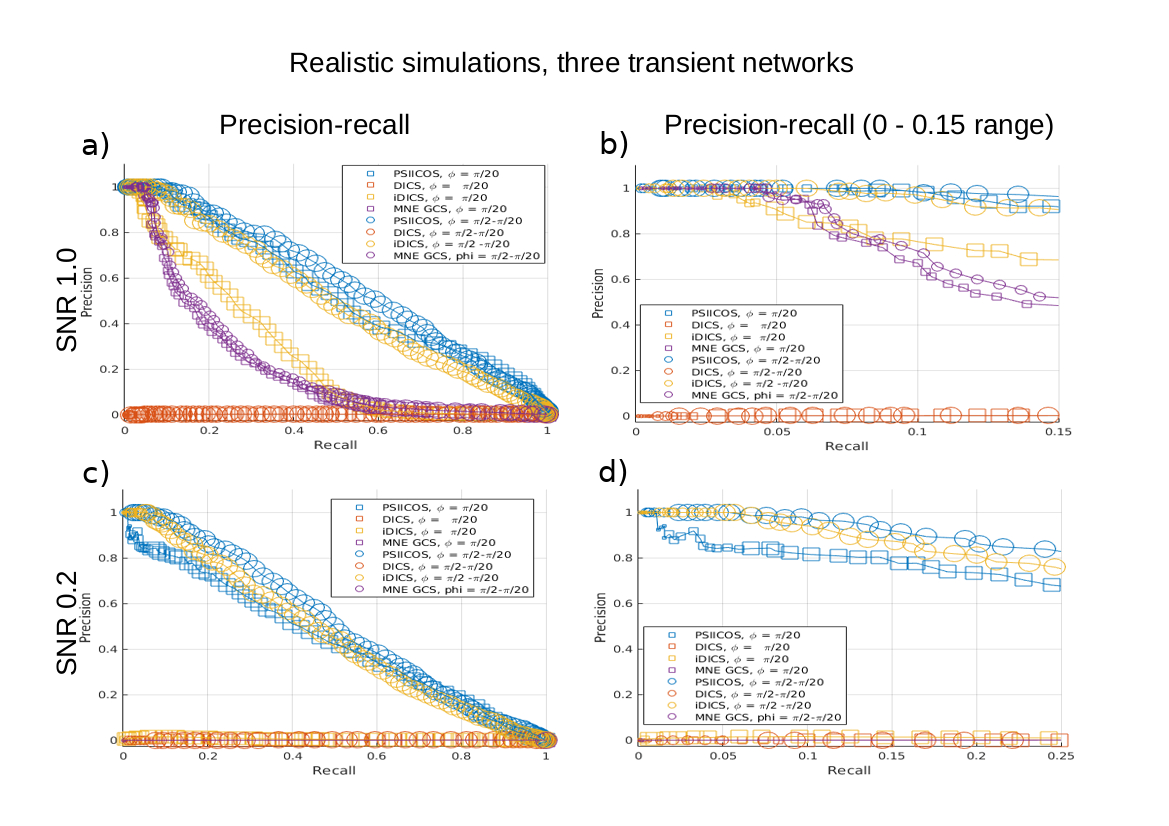
\includegraphics[width=\textwidth]{../images/psiicos_paper/Figure7_hr.jpg}
 % На рисунках (a), (c) изображены кривые Precision-Recall для всего диапазона
 % возможных значений; на рисунках (b), (d) изображены те же кривые, но для
 % диапазона значений 0--0.15.
\end{figure}%
\end{frame}

\begin{frame}{Сравнение PSIICOS c GCS, DICS и iDICS}{для трех сетей с перекрывающимися профилями активации}
\begin{figure}[!ht]
 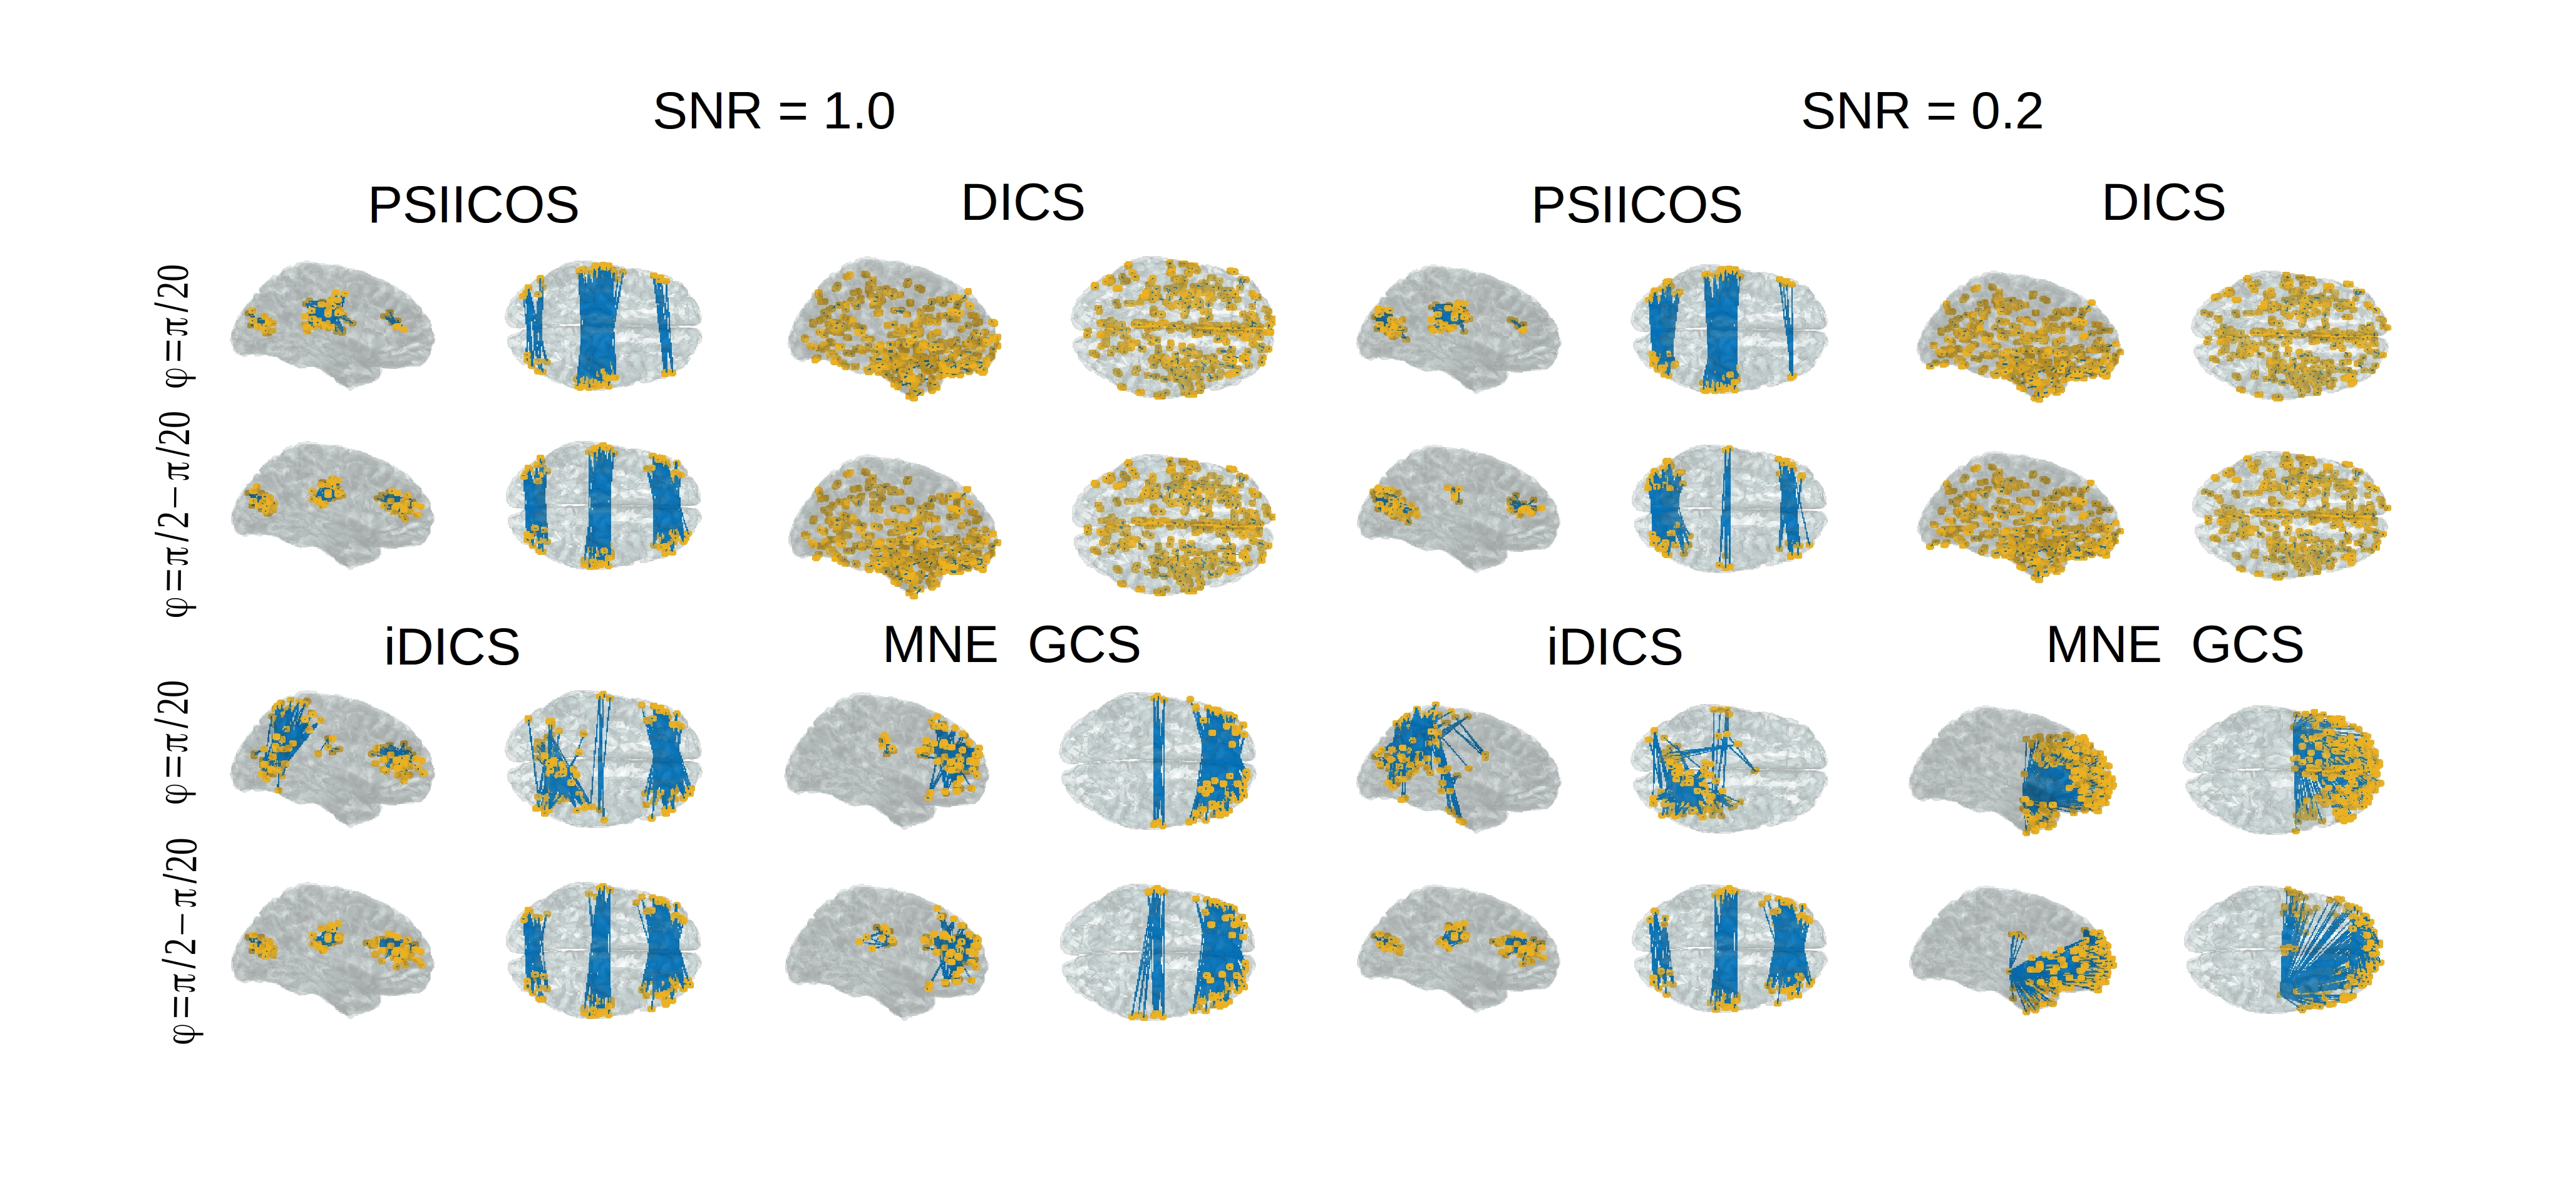
\includegraphics[width=1\textwidth]{../images/psiicos_paper/Figure5_hr.jpg}
 % {\small Пространственное распределение сетевых источников для симуляционных данных.}
     % На графике изображены 0.1\% сетей с наибольшим значением
     % статистики. Из графиков видно, что только алгоритм PSIICOS сохраняет
     % качество решения для всего диапазона изучаемых значений.
     % Метод iDICS ведет себя практически также хорошо, как и PSIICOS,
     % для фазовых сдвигов, близких к $\pi/2$, что согласуется с нашими предыдущими
     % результатами. Метод MNE GCS для высоких значений ОСШ достаточно надежно определяет
     % две фронтальные сети для каждого значения фазового сдвига, но полностью перестает
     % работать для низких значений ОСШ и близких к нулю фазовых задержек. Для задержек,
     % близких к $\pi/2$, при низком ОСШ этот метод находит только среднюю сеть
     % (для нее индивидуальное ОСШ выше всего) а также порождает большое количество
     % ложноположительных срабатываний.
\end{figure}%
\end{frame}

\begin{frame}[t]
    \frametitle{Сравнение PSIICOS и PSIICOS Unbiased}
    \framesubtitle{в задаче детекции сетей со случайными пололжениями узлов}
    \begin{figure}[htbp]
        \begin{subfigure}[t]{0.49\textwidth}
            \centering
            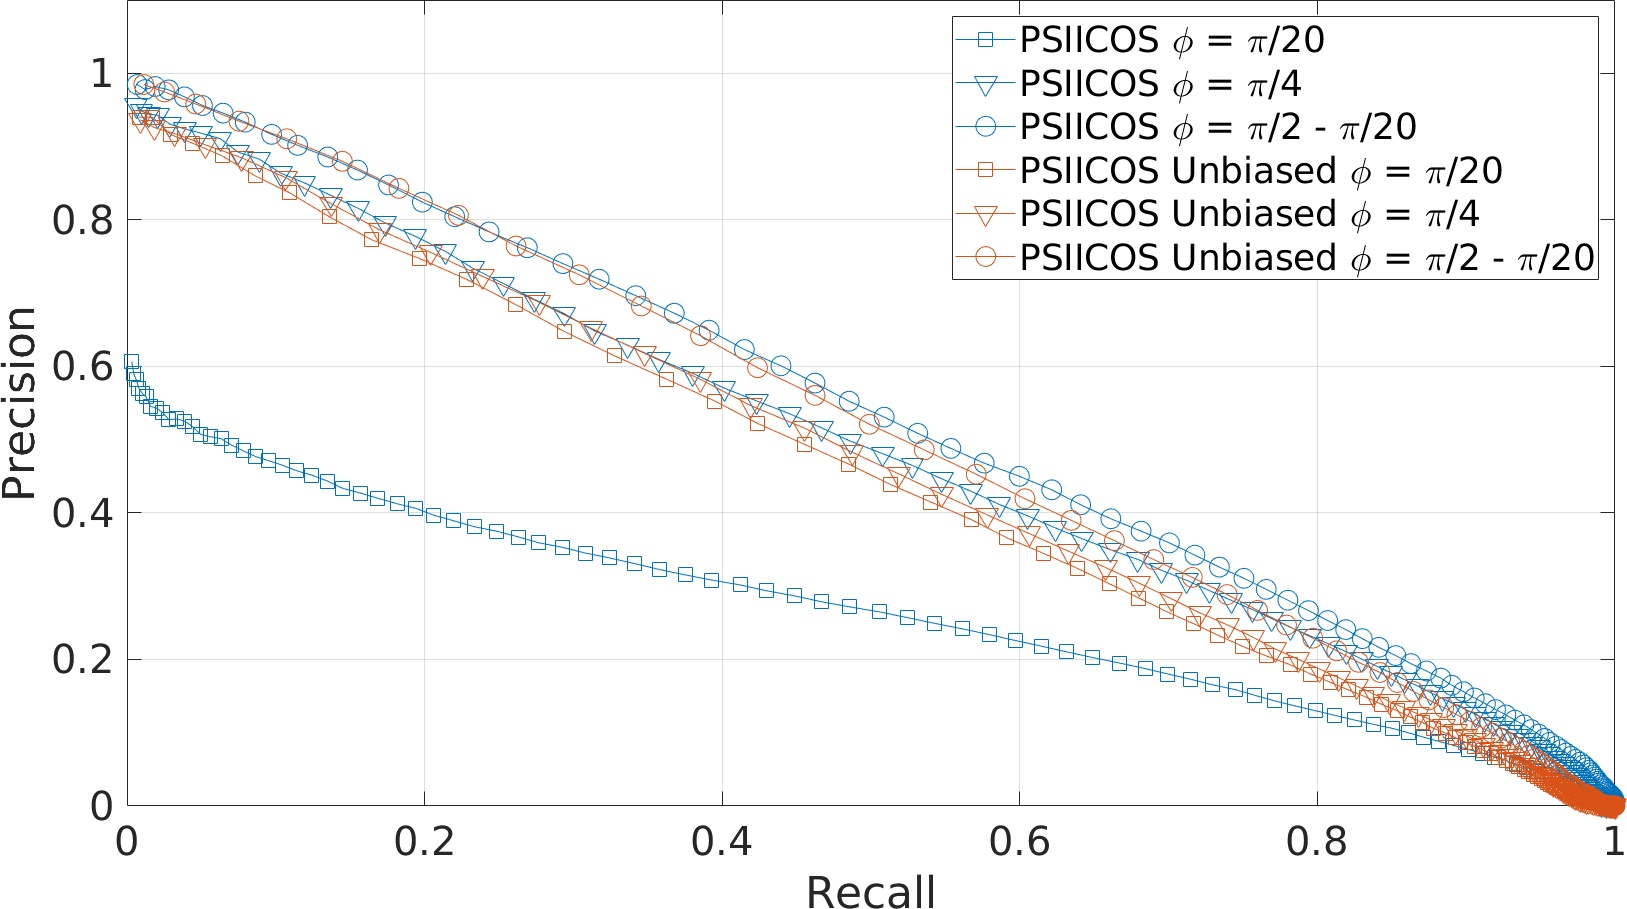
\includegraphics[width=0.9\textwidth]{../images/pre_rec_snr_1.jpg}
            {\tiny Precision-Recall, ОСШ=1}
        \end{subfigure}
            % \hspace{-1.5cm}
        \begin{subfigure}[t]{0.49\textwidth}
            \centering
            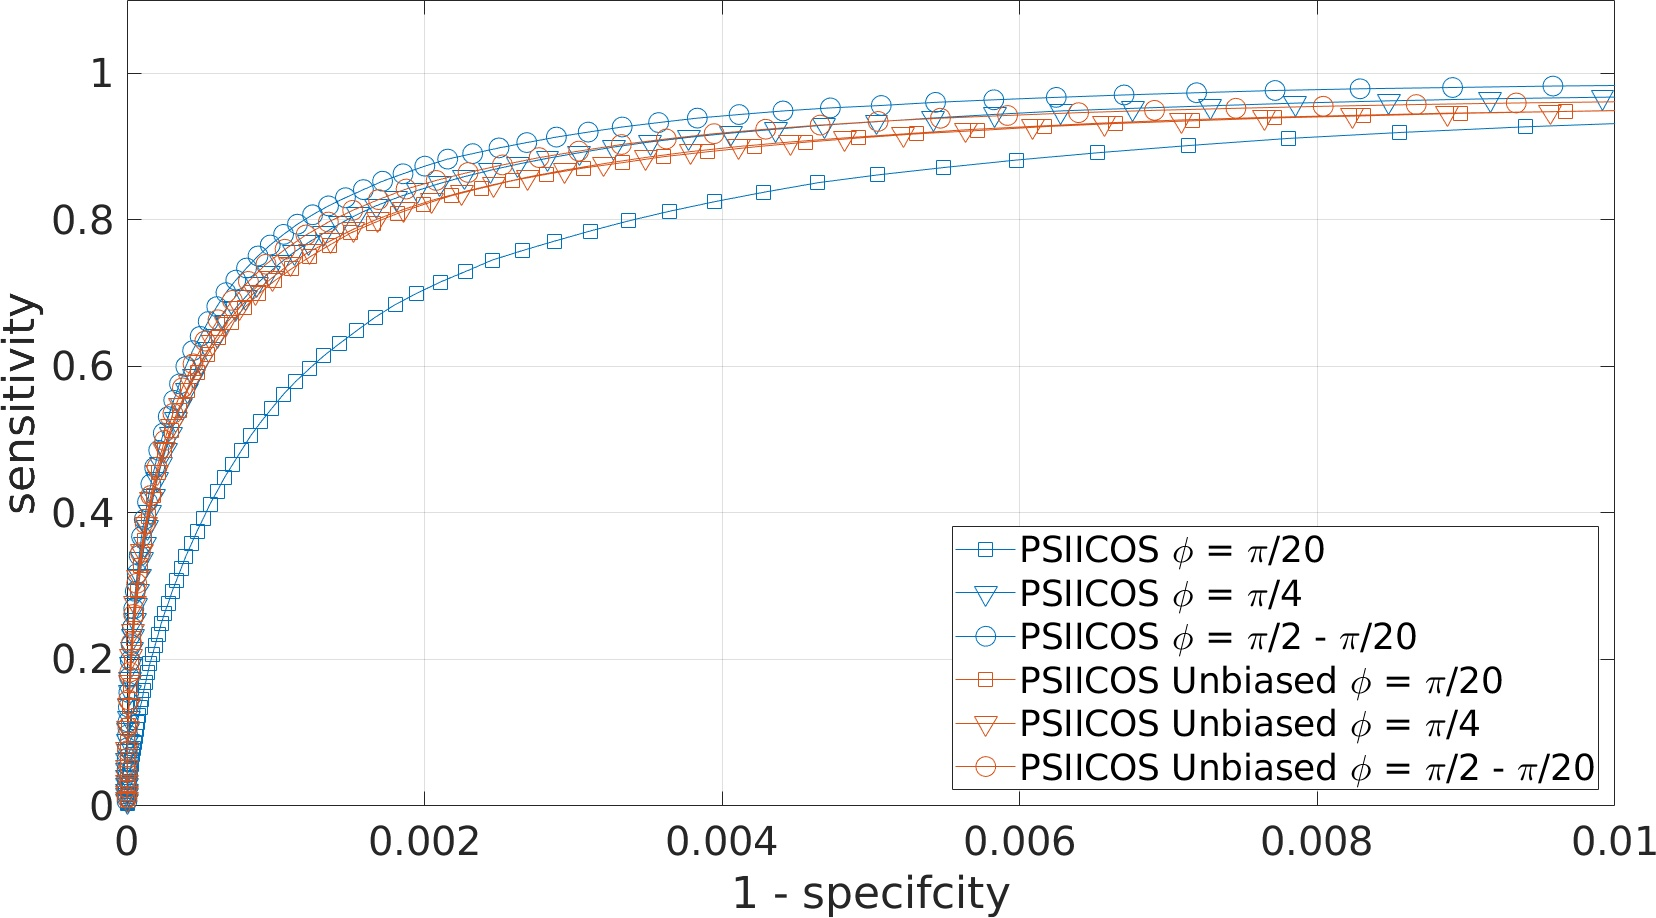
\includegraphics[width=0.9\textwidth]{../images/roc_snr_1.jpg}
            {\tiny ROC, ОСШ=1}
        \end{subfigure}
        % \hspace{-2cm}
        \begin{subfigure}[t]{0.49\textwidth}
            \centering
            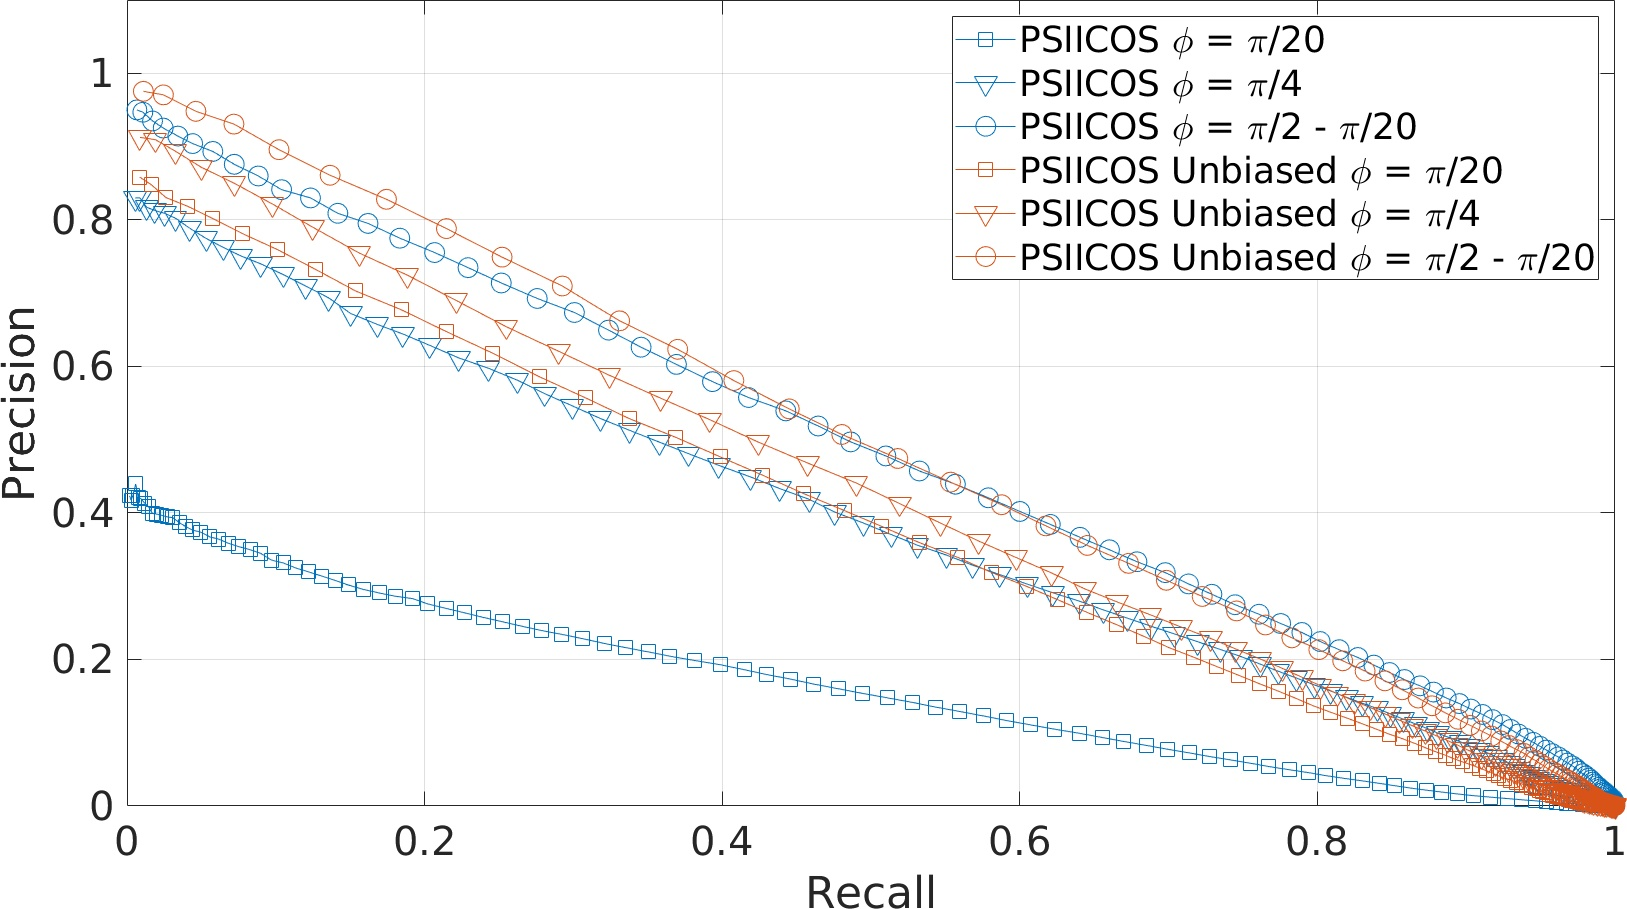
\includegraphics[width=0.9\textwidth]{../images/pre_rec_snr_02.jpg}
            {\tiny Precision-Recall, ОСШ=0.2}
        \end{subfigure}
        \begin{subfigure}[t]{0.49\textwidth}
            \centering
            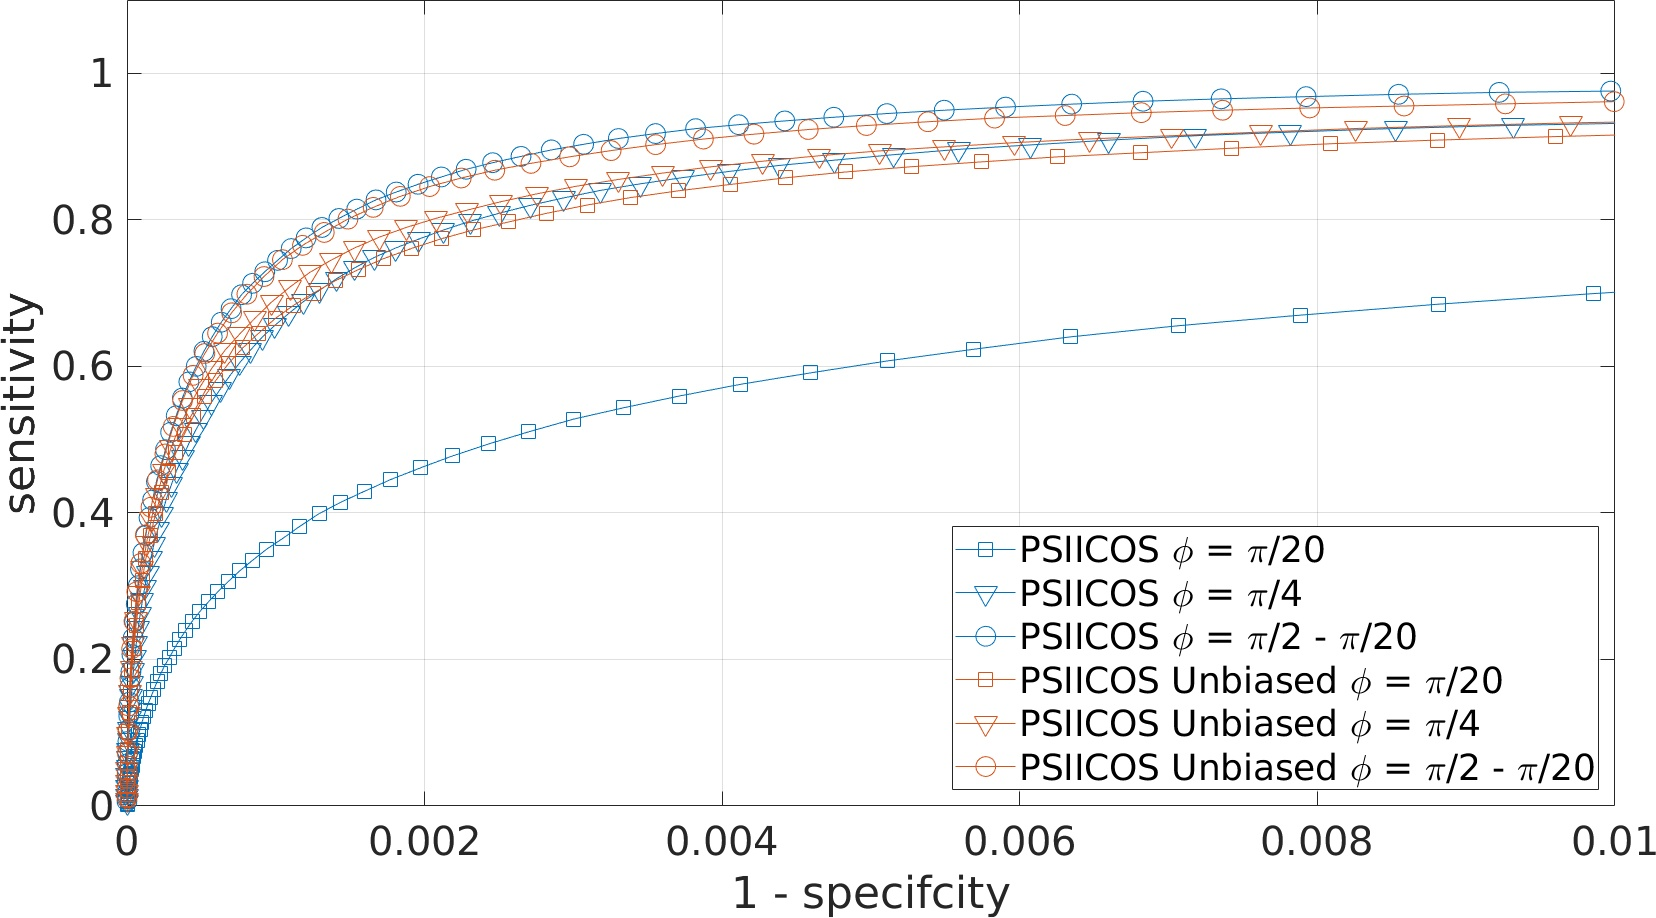
\includegraphics[width=0.9\linewidth]{../images/roc_snr_02.jpg}
            {\tiny ROC, ОСШ=0.2}
        \end{subfigure}
    \end{figure}
\end{frame}


\begin{frame}[t]
    \frametitle{Сравнение PSIICOS и PSIICOS Unbiased}
    
    \vspace{1cm}
    \begin{figure}[htbp]
        \begin{subfigure}[t]{0.49\textwidth}
            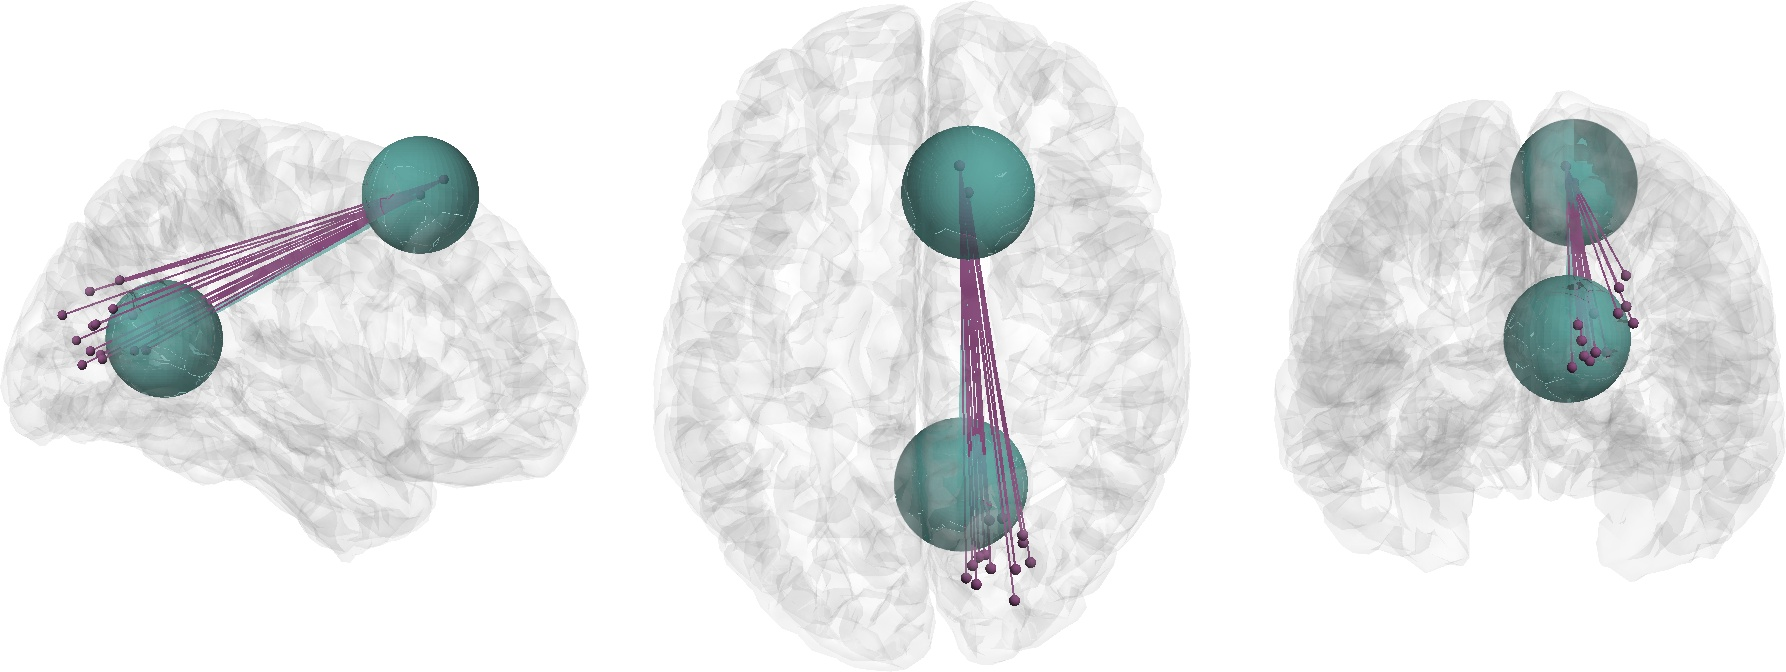
\includegraphics[width=0.99\textwidth]{../images/bias_brain_PSIICOS.jpg}
            \caption{PSIICOS}\label{fig:bias_brain_psiicos}
        \end{subfigure}
        \begin{subfigure}[t]{0.49\textwidth}
            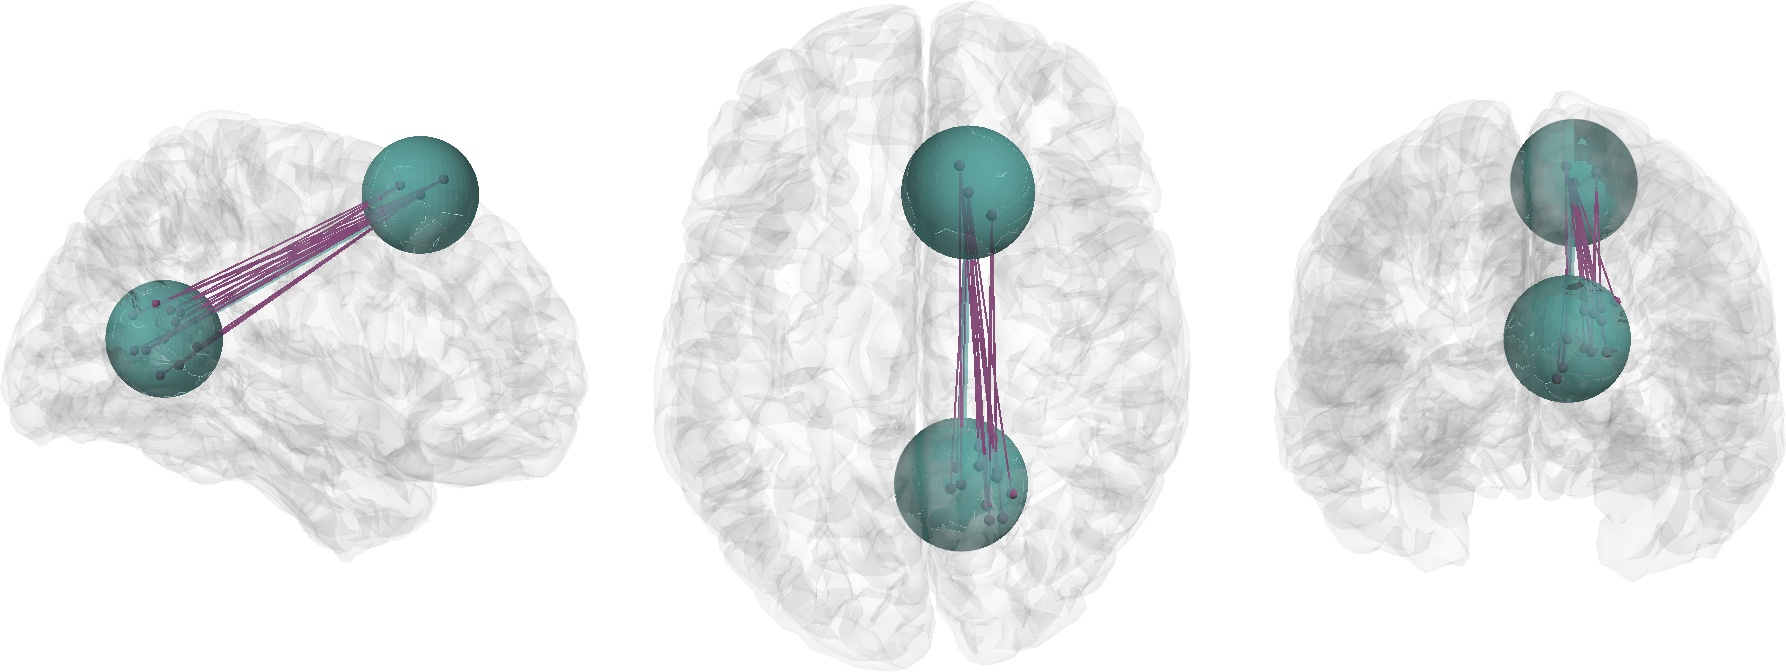
\includegraphics[width=0.99\textwidth]{../images/bias_brain_PSIICOS_Unbiased.jpg}
            \caption{PSIICOS Unbiased}\label{fig:bias_brain_psiicos_unbiased}
        \end{subfigure}
        {\tiny Пример плохого решения для алгоритма PSIICOS по сравнению с
            PSIICOS Unbiased в задаче детекции сетей со случайными положениями
            узлов для одной из итераций Монте-Карло и фазового сдвига
            $\phi=\pi/20$.
        }
        % Фиолетовые отрезки (по 20 для каждого метода)~--- найденные сети; зелеными
        % сферами отмечены зоны, внутри которых найденные сети относились к истинно
        % положительным срабатываниям. Радиус каждой сферы равен 1.8 см.
    \end{figure}

\end{frame}

\begin{frame}[t]
    \frametitle{Сравнение PSIICOS и PSIICOS Unbiased}
    \framesubtitle{в задаче детекции трех сетей с перекрывающимися профилями активации.}
    \vspace{-0.3cm}
    \begin{figure}[htbp]
        \begin{subfigure}[t]{0.49\textwidth}
            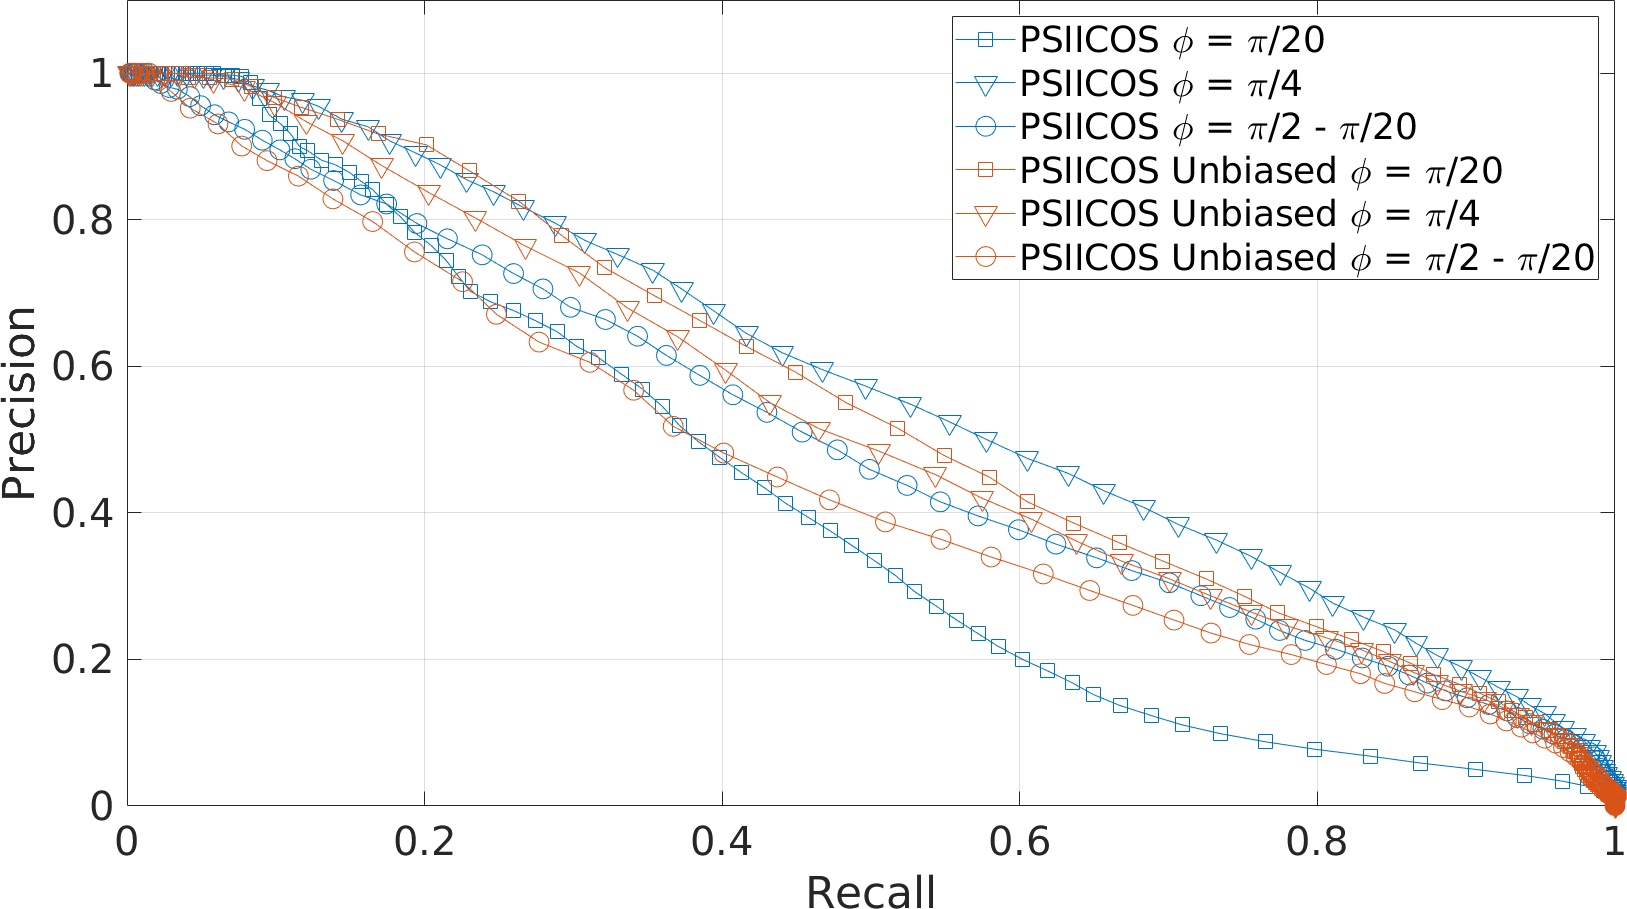
\includegraphics[width=0.99\textwidth]{../images/pre_rec_3_ntw_snr_1.jpg}
            \caption{\tiny Precition-Recall, ОСШ=1}\label{fig:psiicos_vs_unbiased_3_ntw_a}
        \end{subfigure}
        \begin{subfigure}[t]{0.49\textwidth}
            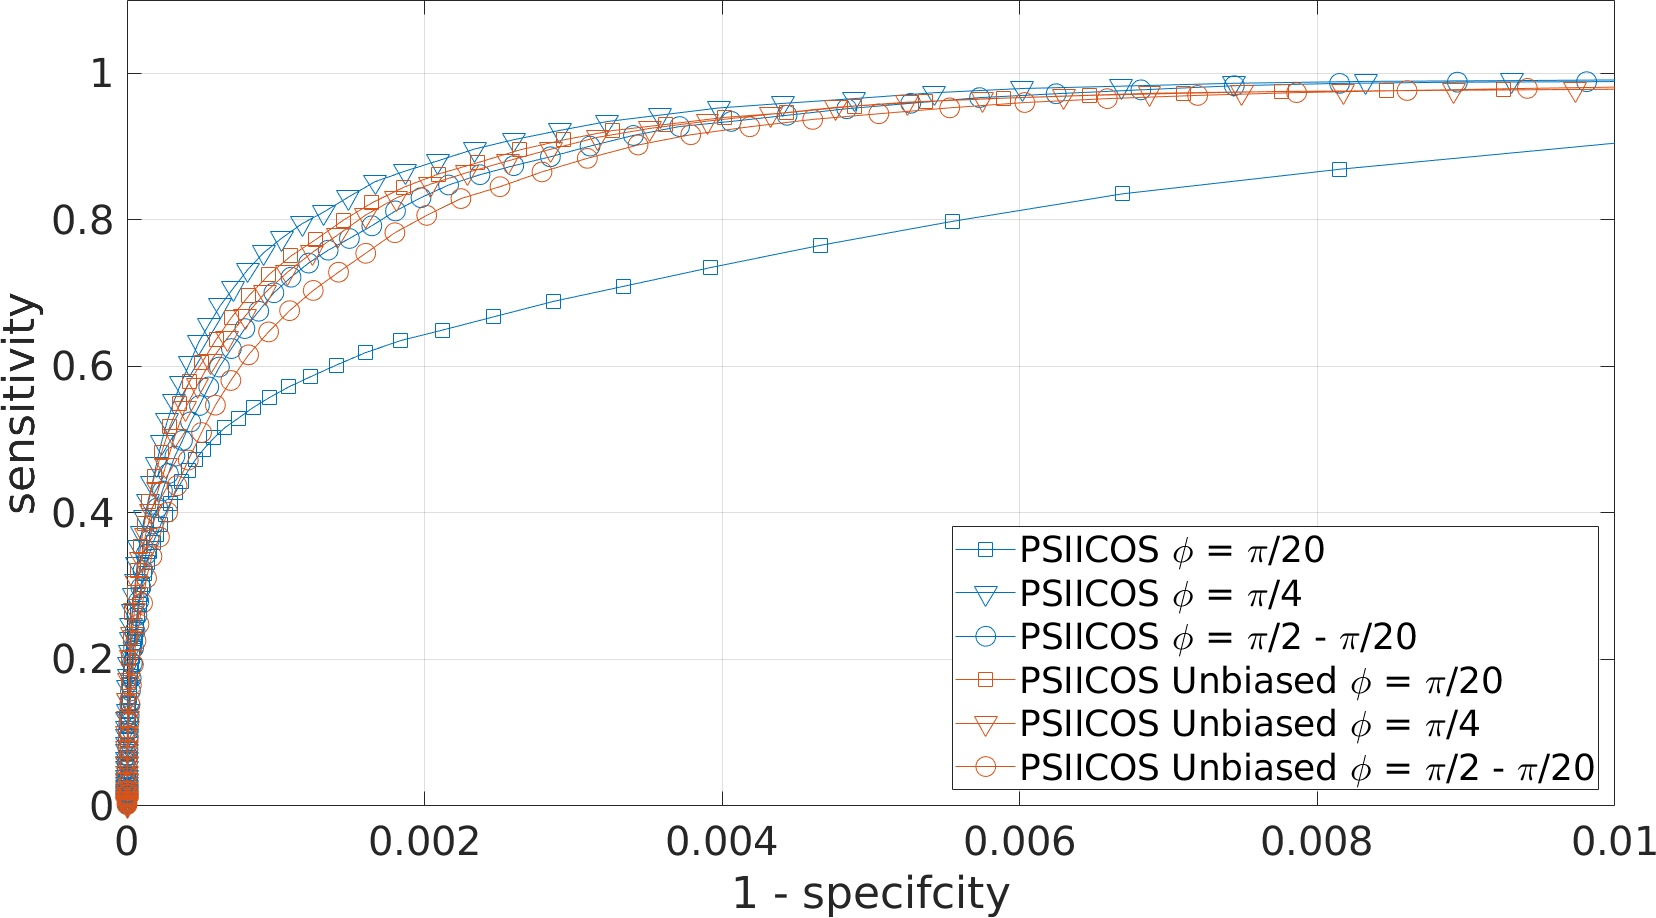
\includegraphics[width=0.99\textwidth]{../images/roc_3_ntw_snr_1.jpg}
            \caption{\tiny ROC, ОСШ=1}\label{fig:psiicos_vs_unbiased_3_ntw_b}
        \end{subfigure}
        \begin{subfigure}[t]{0.49\textwidth}
            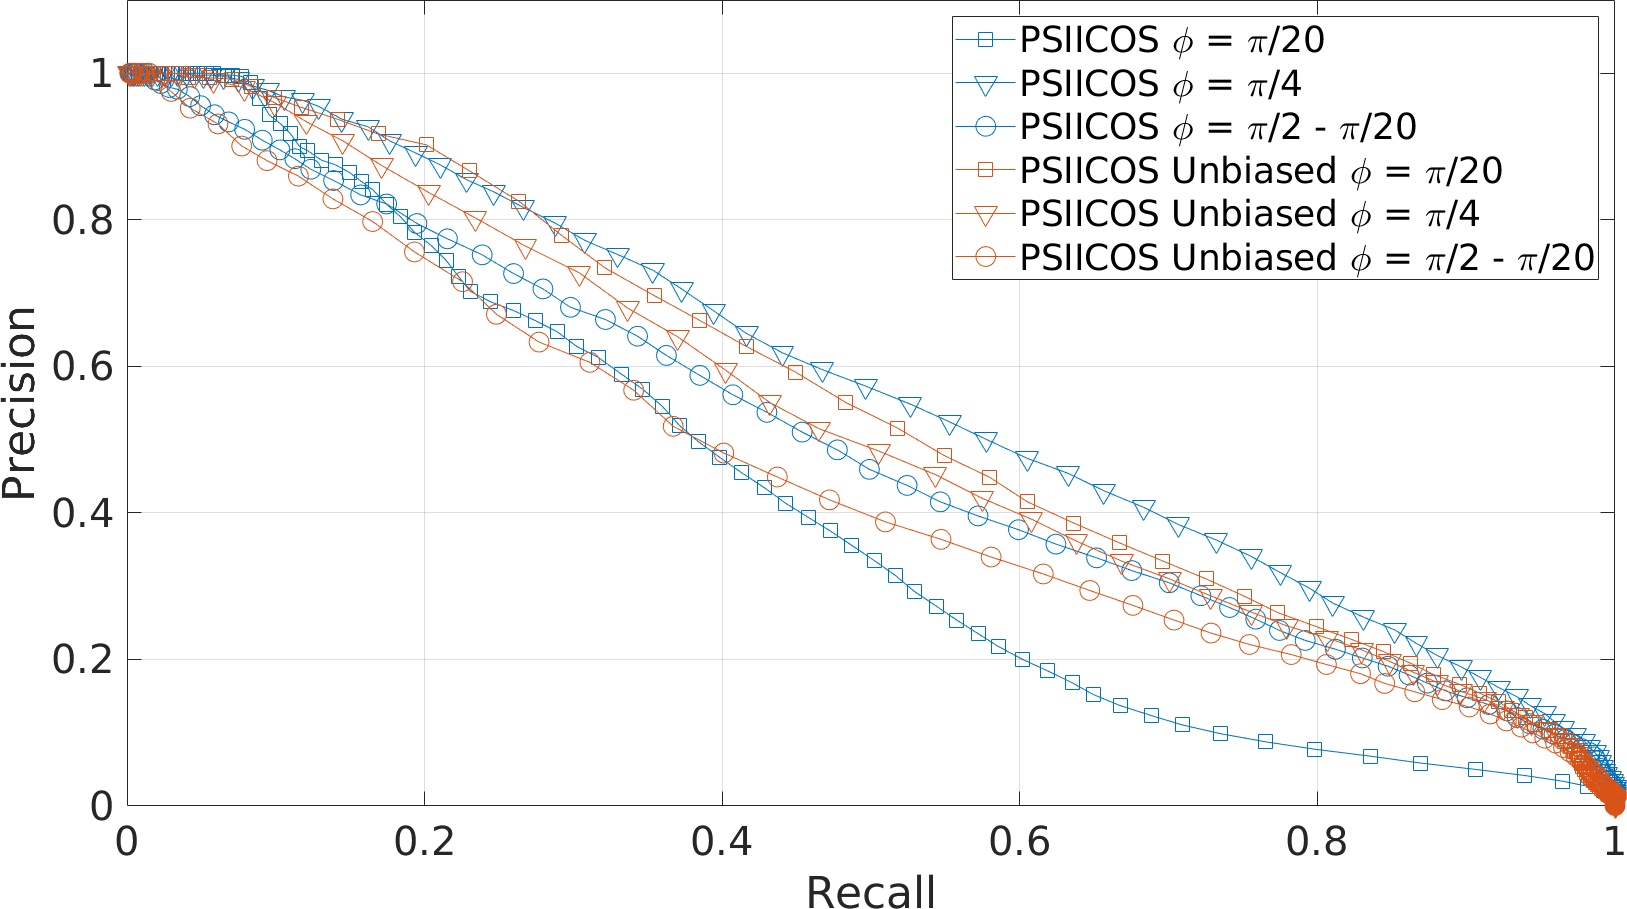
\includegraphics[width=0.99\textwidth]{../images/pre_rec_3_ntw_snr_1.jpg}
            \caption{\tiny Precition-Recall, ОСШ=0.2}\label{fig:psiicos_vs_unbiased_3_ntw_c}
        \end{subfigure}
        \begin{subfigure}[t]{0.49\textwidth}
            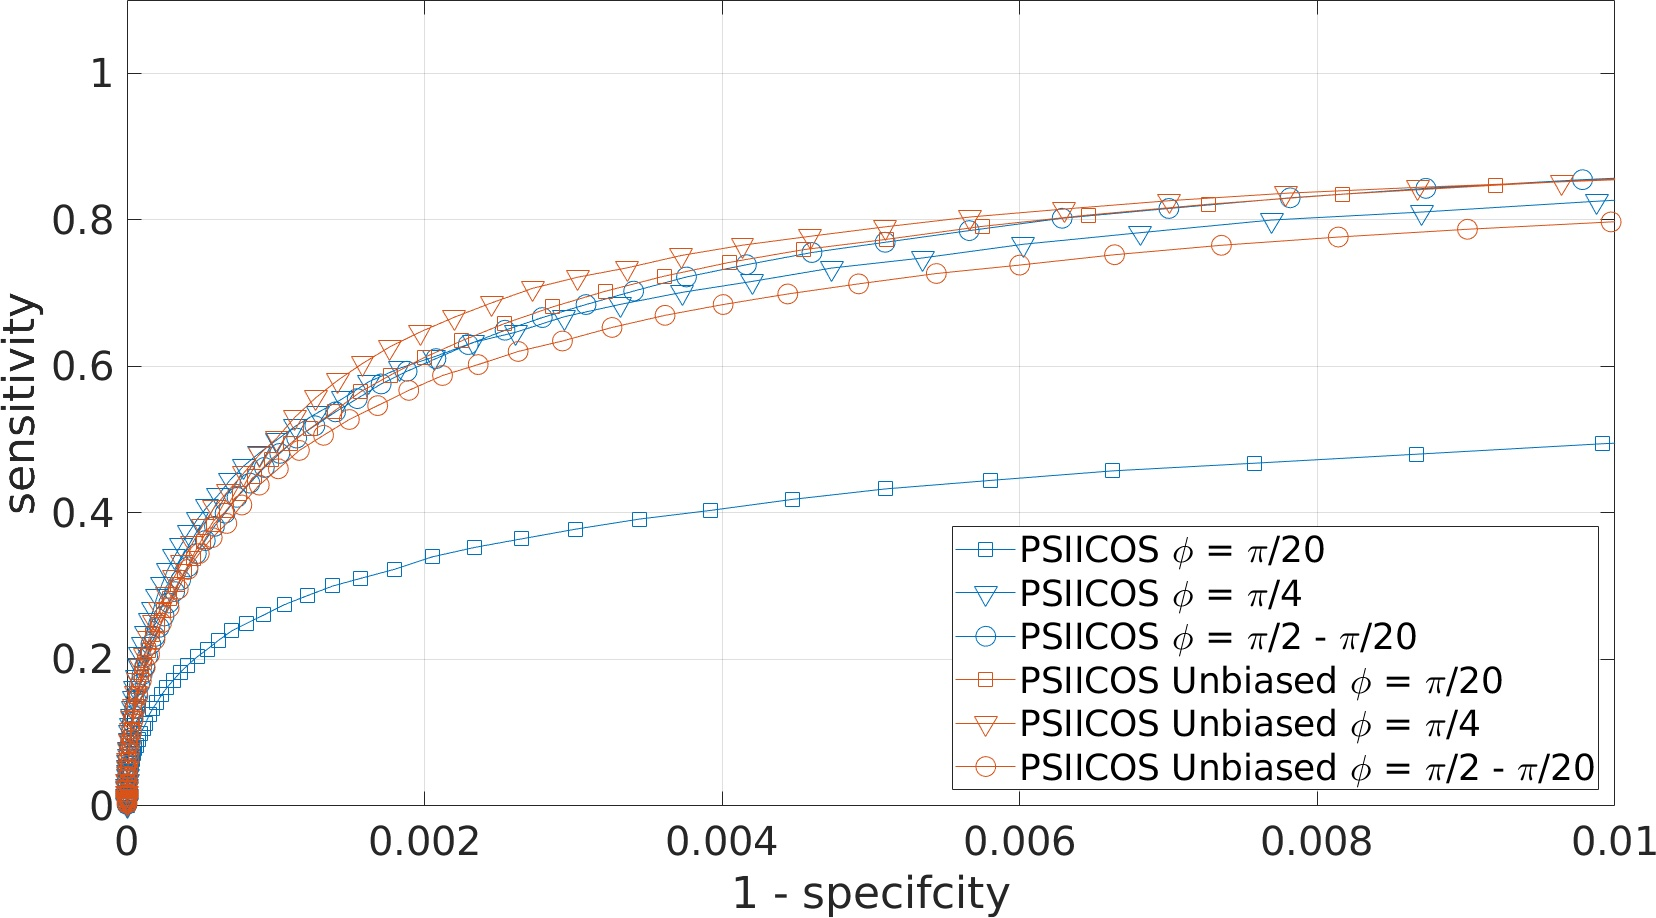
\includegraphics[width=0.99\linewidth]{../images/roc_3_ntw_snr_02.jpg}
            \caption{\tiny ROC, ОСШ=0.2}\label{fig:psiicos_vs_unbiased_3_ntw_d}
        \end{subfigure}
        % \caption{             усредненные по 10 повторениям.}\label{fig:psiicos_vs_unbiased_3_ntw}
    \end{figure}
\end{frame}

\begin{frame}[t]{Мотивация нормализации коэффициентов}{PSIICOS Normalized}
    
    \begin{figure}[htbp]
        \begin{subfigure}[t]{0.245\textwidth}
            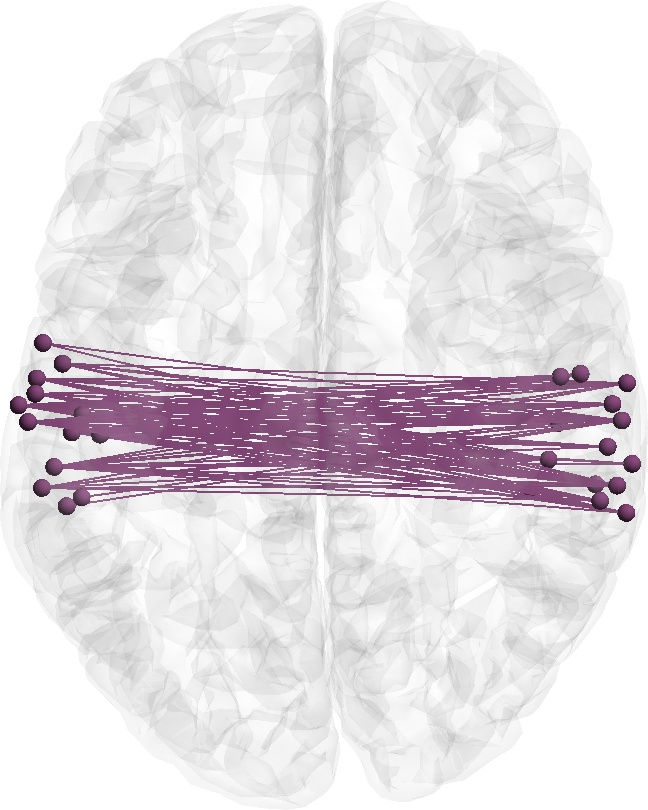
\includegraphics[width=0.99\textwidth]{../images/loreta_brain_jitter_01_snr_02_phase_lag_07854.jpg}
            \caption{\tiny $\alpha=0.1$, ОСШ=0.2}\label{fig:unbiased_1_ntw_a}
        \end{subfigure}
        \begin{subfigure}[t]{0.24\textwidth}
            \includegraphics[width=0.99\linewidth]{../images/loreta_brain_jitter_2_snr_02_phase_lag_07854.jpg}
            \caption{\tiny $\alpha=2$, ОСШ=0.2}\label{fig:unbiased_1_ntw_b}
        \end{subfigure}
        \begin{subfigure}[t]{0.24\textwidth}
            \includegraphics[width=0.99\textwidth]{../images/loreta_brain_jitter_01_snr_1_phase_lag_07854.jpg}
            \caption{\tiny $\alpha=0.1$, ОСШ=1}\label{fig:unbiased_1_ntw_c}
        \end{subfigure}
        \begin{subfigure}[t]{0.235\textwidth}
            \includegraphics[width=0.99\linewidth]{../images/loreta_brain_jitter_2_snr_1_phase_lag_07854.jpg}
            \caption{\tiny $\alpha=2$, ОСШ=1}\label{fig:unbiased_1_ntw_d}
        \end{subfigure}

        {\tiny\centering Локализация сети с фиксированными положениями узлов методом PSIICOS Unbiased для 
        фазового сдвига $\phi=\pi/4$ для высокого и низкого ОСШ (0.2 и 1) в
        случае сильной связности ($\alpha=0.1$) и отсутствия связности ($\alpha=2$)}\label{fig:unbiased_breaks_in_high_snr}

        {\footnotesize PSIICOS Normalized --- модификация метода PSIICOS Unbiased, которая позволяет получать нормированные коэффициенты кросс-спектра}
    \end{figure}
\end{frame}


\begin{frame}[t]
    
\begin{figure}[htbp]
    \begin{subfigure}[t]{0.49\textwidth}
        \includegraphics[width=0.99\textwidth]{../images/bars_snr_02.jpg}
        \caption{ОСШ=0.2}\label{fig:bars_a}
    \end{subfigure}
    \begin{subfigure}[t]{0.49\textwidth}
        \includegraphics[width=0.99\linewidth]{../images/bars_snr_1.jpg}
        \caption{ОСШ=1}\label{fig:bars_b}
    \end{subfigure}
    {\footnotesize Нормализованный индекс фазовой связности, полученный методом
    PSIICOS Normalized для одной симулированной сети в условиях высокого и низкого ОСШ
    в зависимости от индекса истинной фазовой связности $\alpha$ и значения
    фазовой задержки.}
\end{figure}

\end{frame}

\begin{frame}[t]
    \frametitle{Применение метода GO-PSIICOS}
    \framesubtitle{симуляционные данные, 3 сети}
    
\begin{figure}[htbp]
    \centering
    \begin{columns}
        \begin{column}{0.12\textwidth}
            \tiny
            $\pi/20$
            \vspace{1.6cm}

            $\pi/4$
            \vspace{1.6cm}

            $\pi/2 - \pi/20$
        \end{column}
    \hspace{-1cm}
    \begin{column}{0.59\textwidth}
    \centering
        \includegraphics[width=0.7\textwidth]{../images/networks_gopsiicos.jpg}
        \includegraphics[width=0.7\textwidth]{../images/networks_gopsiicos_pi4.jpg}
        \includegraphics[width=0.7\textwidth]{../images/networks_gopsiicos_pi2pi20.jpg}
        % \caption{\tiny \Восстановленные сети, $\phi=\pi/20$}\label{fig:gopsiicos_a}
    \end{column}
    \hspace{-1.2cm}
    \begin{column}{0.39\textwidth}
    \centering
        \includegraphics[width=0.7\linewidth]{../images/timeseries_gopsiicos.jpg}
        \includegraphics[width=0.7\linewidth]{../images/timeseries_gopsiicos_pi4.jpg}
        \includegraphics[width=0.7\linewidth]{../images/timeseries_gopsiicos_pi2pi20.jpg}
    \end{column}
    % \begin{column}{0.59\textwidth}
    %     % {\tiny $\phi=\pi/4$}\label{fig:gopsiicos_c}
    % \centering
    % \end{column}
    % \begin{column}{0.39\textwidth}
    % \centering
    % \end{column}
    % \begin{column}{0.59\textwidth}
    % \centering
    %     % \caption{\tiny Восстановленные сети, $\phi=\pi/2-\pi/20$}\label{fig:gopsiicos_e}
    % \end{column}
    % \begin{column}{0.39\textwidth}
    \centering
    % \end{column}
\end{columns}
{\footnotesize Детекция перекрывающихся во времени сетей методом GO-PSIIOCS, ОСШ=0.5}
\end{figure}
\end{frame}

\begin{frame}[t]
    \frametitle{Применение метода PSIICOS к реальным данным}
    
    \vspace{1cm}
    \centering
    {\small Задача воображения вращения руки (\cite{DeLangeHensen2008}):}

    \includegraphics[width=1\textwidth]{./real_data.png}
    {\tiny Необходимо по повернутому изображению руки определить ее латеральность.}
    {\tinyДанные для одного испытуемого из исследования \cite{DeLangeHensen2008} были опубликованы в ходе соревнования по анализу данных на конференции Biomag 2010}
\end{frame}

\begin{frame}[t]{Анализ воспроизводимости сетей}{на реальных данных}
    \vspace{1cm}
    \begin{figure}[h!tpb]
     \includegraphics[width=1\textwidth]{../images/psiicos_paper/Figure10_hr.jpg}
     {\small Полосы частот с наиболее воспроизводимыми сетями, определенными при помощи
     процедуры бутстрэпа.}
     % Бутстрэп проводился последовательным выбором подмножества эпох, на котором
     % вычислялся кросс-спектр, к которому затем применялась PSIICOS-проекция.
     % Столбики на графике отображают индекс воспроизводимости, который вычислялся
     % как обратное к среднему расстоянию до ближайшего соседа для каждой отдельной
     % сети, найденной по мнимой и действительной спроецированной части кросс-спектра для четырех
     % наиболее значимых главных компонент. Результаты для действительной части представлены
     % синим цветом, а для мнимой~--- желтым.
     \end{figure} %Figure 10
\end{frame}


\begin{frame}[t]{Бутстрэп-решения для воспроизводимых сетей}
    % \framesubtitle{subtitle}
    \begin{figure}
    \centering
    \text{\small Тета- (3--6 Гц) и альфа- (8--12 Гц) диапазоны}

     \begin{subfigure}[b]{0.47\textwidth}
     \includegraphics[width=\textwidth]{../images/psiicos_paper/Figure11_a1.jpg}
     \includegraphics[width=\textwidth]{../images/psiicos_paper/Figure11_a2.jpg}
     {\small Тета-диапазон, Re, сеть 1}\label{fig:11a}
     \end{subfigure}
     \hspace{0.2cm}
     \begin{subfigure}[b]{0.47\textwidth}
     \includegraphics[width=\textwidth]{../images/psiicos_paper/Figure11_b1.jpg}
     \includegraphics[width=\textwidth]{../images/psiicos_paper/Figure11_b2.jpg}
     {\small Альфа-диапазон, Im, сеть 1}\label{fig:11b}
     \end{subfigure}
     % \caption{Пространственная структура и временная динамика наиболее воспроизводимых сетей в диапазонах частот тета (3--6 Гц) и альфа (8--12 Гц)}\label{fig:11}
    \end{figure} % figure 11
\end{frame}

\begin{frame}[t]
    \frametitle{Бутстрэп-решения для воспроизводимых сетей}
    
    \begin{figure}
    \centering
    \text{Бета-диапазон (16--24 Гц)}

     \begin{subfigure}[b]{0.4\textwidth}
     \includegraphics[width=\textwidth]{../images/psiicos_paper/Figure12_a1.jpg}
     \includegraphics[width=\textwidth]{../images/psiicos_paper/Figure12_a2.jpg}
     \caption{Re, сеть 1}\label{fig:12a}
     \end{subfigure}
     \hspace{1cm}
     \begin{subfigure}[b]{0.4\textwidth}
     \includegraphics[width=\textwidth]{../images/psiicos_paper/Figure12_b1.jpg}
     \includegraphics[width=\textwidth]{../images/psiicos_paper/Figure12_b2.jpg}
     \caption{Re, сеть 2}\label{fig:12b}
     \end{subfigure}
     \begin{subfigure}[b]{0.4\textwidth}
     \includegraphics[width=\textwidth]{../images/psiicos_paper/Figure12_c1.jpg}
     \includegraphics[width=\textwidth]{../images/psiicos_paper/Figure12_c2.jpg}

     \caption{Im, сеть 1}\label{fig:12c}
     \end{subfigure}
     \caption{Пространственная структура и временная динамика наиболее воспроизводимых сетей в бета-диапазоне (16--24 Гц)}\label{fig:12}
    \end{figure} %figure 12
\end{frame}

\begin{frame}[t]
    \frametitle{Реальные данные}
    % \framesubtitle{subtitle}
    \begin{figure}
    \centering
    \text{\tiny Нижний (30--60 Гц) и верхний (65--85 Hz) гамма-диапазоны}
     \begin{subfigure}[b]{0.4\textwidth}
     \includegraphics[width=\textwidth]{../images/psiicos_paper/Figure13_a1.jpg}
     \includegraphics[width=\textwidth]{../images/psiicos_paper/Figure13_a2.jpg}
     \caption{\tiny Ниж. гамма-диапазон, Re, сеть 1}\label{fig:13a}
     \end{subfigure}
     \hspace{1cm}
     \begin{subfigure}[b]{0.4\textwidth}
     \includegraphics[width=\textwidth]{../images/psiicos_paper/Figure13_b1.jpg}
     \includegraphics[width=\textwidth]{../images/psiicos_paper/Figure13_b2.jpg}
     \caption{\tiny Верх. гамма-диапазон, Re, сеть 1}\label{fig:13b}
     \end{subfigure}

     \begin{subfigure}[b]{0.4\textwidth}
     \includegraphics[width=\textwidth]{../images/psiicos_paper/Figure13_c1.jpg}
     \includegraphics[width=\textwidth]{../images/psiicos_paper/Figure13_c2.jpg}
     \caption{\tiny Ниж. гамма-диапазон, Im, сеть 1}\label{fig:13c}
     \end{subfigure}
     % \caption{Пространственная структура и временная динамика наиболее воспроизводимых сетей в нижнем (30--60 Гц) и верхнем (65--85 Гц) гамма-диапазонах}\label{fig:13}
    \end{figure} % Figure 13
\end{frame}








%%%%%%%%%%%%%%%%%%%%%%%%%%%%%%

\begin{frame}[t]
    \frametitle{Результаты работы}
    Для~достижения поставленных целей необходимо было решить следующие задачи:
    \begin{enumerate}
    \tiny
      \item Разработать методику очистки сигнала от объемной проводимости
      \item Исследовать свойства методики очистки сигнала
            для сетей с малым и большим фазовым сдвигом;
            сравнить с методиками, описанными в литературе.
      \item Разработать методологию оптимального оценивания достаточной статистики
            для фазовых синхронностей.
      \item Реализовать алгоритм оценивания, позволяющий использовать спарсную регуляризацию
      \item Разработать код для численного решения задачи невыпуклой оптимизации
      \item Разработать методику визуализации найденных сетей.
      \item Разработать методологию генерации данных, симулирующих мозговую активность
      \item Сравнить детекторные характеристики разработанного метода на симуляционных данных
            по стандартным метриках (AUC-ROC, AUC-Pre-Rec)
    \end{enumerate}
\end{frame}

\begin{frame}{Результаты работы.}{Положения, выносимые на защиту.}
\begin{enumerate}
    \footnotesize
  \item Разработан метод, позволяющий обнаруживать связанные по фазе источники с околонулевыми фазовыми задержками
      по неинвазивным МЭГ-записям. Суть метода заключается в построении пространственного фильтра,
      действующего в пространстве векторизованных матриц кросс-спектральной плотности мощности,
      который позволяет подавить вклад членов, ответственных за эффект протечки сигнала, маскирующий
      информацию о взаимодействии с околонулевой фазой.
  \item Показана оптимальность предложенного фильтра с точки зрения удаления вклада третих источников
      в оценку фазовой связности для фиксированной сети.
  \item На основе метода глобальной оптимизации IrMxNE и предложенного фильтра разработан метод,
      устойчивый к протечке сигнала на уровне сетей и на уровне источников. Первое обеспечивается
      спарсными свойствами метода IrMxNE, второе~--- свойствами разработанного фильтра.
\end{enumerate}
\end{frame}

\begin{frame}
\frametitle{Перспективы развития предложенных методов}
\begin{itemize}
    \footnotesize
  \item Использование анатомической информации для построения априорных распределений сетей в методе GO-PSIICOS.
      Например, данных диффузионного МРТ.
  \item Исследование возможности построения адаптивных фильтров, подавляющих взаимную протечку сигнала с учетом
      пространственного распределения мощности источников.
  \item Исследование методов на реальных данных с известным распределением коннективности, полученным
    с применением интракраниальных записей.
\end{itemize}
\end{frame}

\begin{frame}
\begin{center}
Спасибо за внимание!
\end{center}
\end{frame}

\begin{frame}[t]
    \vspace{2cm}
    \frametitle{Ссылки на реализацию алгоритмов}
    \begin{itemize}
        \item Вспомогательные утилиты: https://github.com/dmalt/utils\_psiicos
        \item PSIICOS, PSIICOS Unbiased, PSIICOS Normalized: https://github.com/dmalt/PSIICOS
        \item GO-PSIICOS: https://github.com/dmalt/go-psiicos
    \end{itemize}
\end{frame}

\begin{frame}[t,allowframebreaks]{Список литературы}
    \tiny
    \bibliographystyle{plainnat}
    
    \bibliography{binding_refs}
\end{frame}

\begin{frame}[t]{Влияние ранга проекции}{на качество решений}
    \begin{figure}[htbp]
    \includegraphics[width=\textwidth]{../images/psiicos_paper/Figure14_hr.jpg}
    {\footnotesize(a) Ослабление мощности в подпространствах $S_{SL}$ и $S_{Re}$ и\\
        (b) Разница в коэффициенте затухания для подпространств $S_{Re}$ и $S_{SL}$ как
        функции ранга проекции для трех различных размерностей пространства виртуальных
        сенсоров (VS).
    }\label{fig:14}
        % Эти кривые позволяют принять обоснованное решение
        % относительно выбора ранга проекции.  Мы предлагаем выбирать такое значение ранга
        % проекции PSIICOS, которое соответствует наибольшей разнице в затухании
        % мощности.
    \end{figure}
\end{frame}

\begin{frame}[t]
    \frametitle{Влияние шума в прямой модели на качество проекции.}
    \begin{figure}[htbp]
    \includegraphics[width=1\textwidth, height=7cm]{../images/psiicos_paper/Figure15_hr.jpg}
      % На панели (a) изображена зависимость коэффициента затухания от интенсивности шума $\alpha$.
      % Панель (b) показвает коэффициент ослабления мощности в подпространстве $S_{\Re}$.
      % На панели (с) нарисовано подавление мощности в подпространстве SL по сравнению с мощностью в $S_{\Re}$.
      % Как видим, оно монотонно убывает с ростом интенсивности шума в прямой модели.
 \end{figure}
\end{frame}

\begin{frame}
\begin{figure}[!ht]
    \includegraphics[width=1\textwidth]{../images/psiicos_paper/Figure6_hr.jpg}
    {\small Временные профили активации симулированных сетей, восстанновленные при помощи PSIICOS, для двух значений фазового сдвига и двух значений ОСШ.} %Figure 6
        % Непрерывные линии отображают истинные симулированные профили, а
        % пунктир~--- восстановленные алгоритмом PSIICOS.\@
\end{figure}%
\end{frame}

\begin{frame}
\begin{figure}[!ht]
 \includegraphics[width=\textwidth]{../images/psiicos_paper/Figure8_hr.jpg}
 {\small Исследование стабильности метода PSIICOS при помощи процедуры бутстрэпа для
 двух значений фазового сдвига и двух ОСШ.}\label{fig:08}
 % (a), (b), (d), (f)~--- стабильные сети отображены в виде отрезков, концы которых
 % соответствуют взаимодействующим областям коры. Насыщенность цвета отрезка
 % и его концов прямо пропорциональна коэффициенту воспроизводимости $\eta$,
 % оцененному при помощи процедуры бутстрэпа. Отрезки, концы которых
 % оказывались ближе 1 см друг к другу, мы рисовали одним цветом.
 % На графиках (c) и (d) изображен индекс воспроизводимости $\eta$ для
 % двух средних фазовых сдвигов, полученных в результате описанной процедуры
 % бутстрэпа для двух различных значений ОСШ (ОСШ=0.2 и ОСШ=1 соответственно).
\end{figure}% Figure 8
\end{frame}

\end{document} 
